\chapter{Discriminative Models to Predict Stopout} \label{chap:logreg}

In the Chapter \ref{chap:features} we presented the feature extraction process, where a feature represents student behavior on a weekly basis. There are $m$ \feat per student, which we assemble as shown in the figure below: 

\begin{figure}[ht!]
  \caption{The feature matrix, which captures each feature value for each week. Each student has such a matrix.}\label{fig:student_weekly_features}
  \centering
    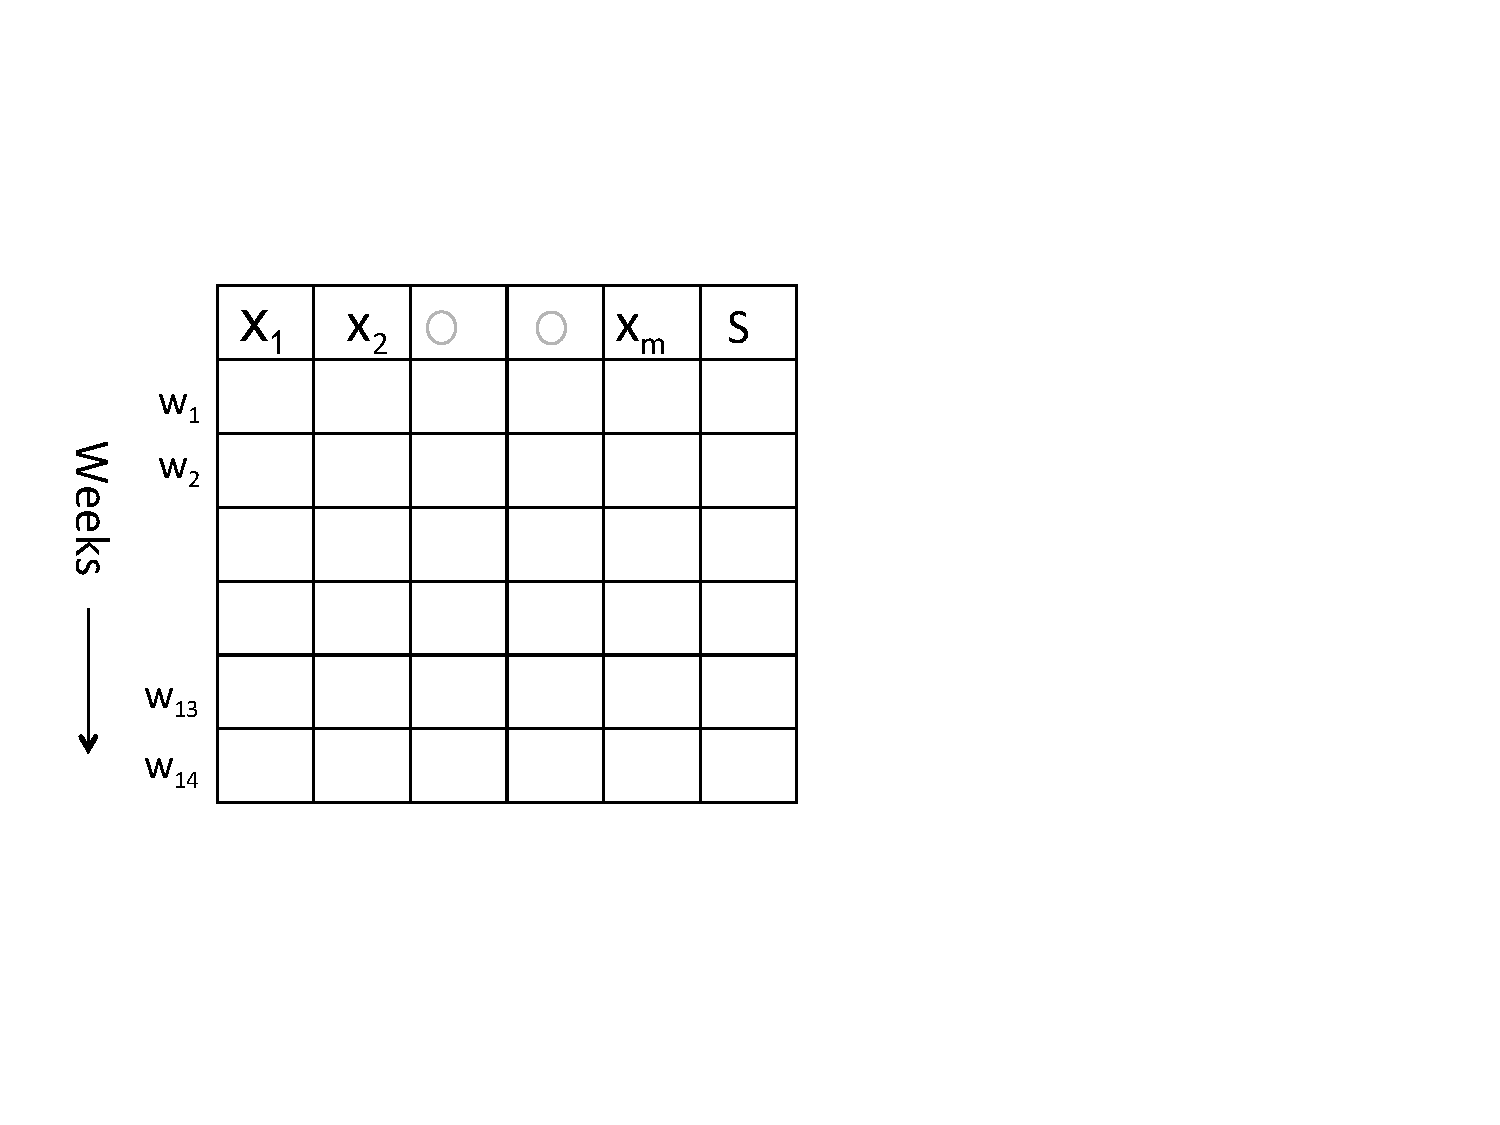
\includegraphics[width=0.5\textwidth]{figures/student_week_matrix}
\end{figure}

To illustrate the predictive model's potential application, we will use a realistic scenario. The model user, likely an instructor or platform provider, could use the data from week 1 to week $i$ (current week) to make predictions. The model will predict existing student \sti during weeks $i+1$ to $14$. For example, Figure~\ref{fig:lead_lag2} shows one such prediction problem. In this case the user, currently at the end of week 3, is attempting to predict \sti for the 8th week. 
\begin{figure}[!ht]
  \caption{Diagram of the student's weeks data used in a lead 5, \lag 3 prediction problem}\label{fig:lead_lag2}
  \centering
    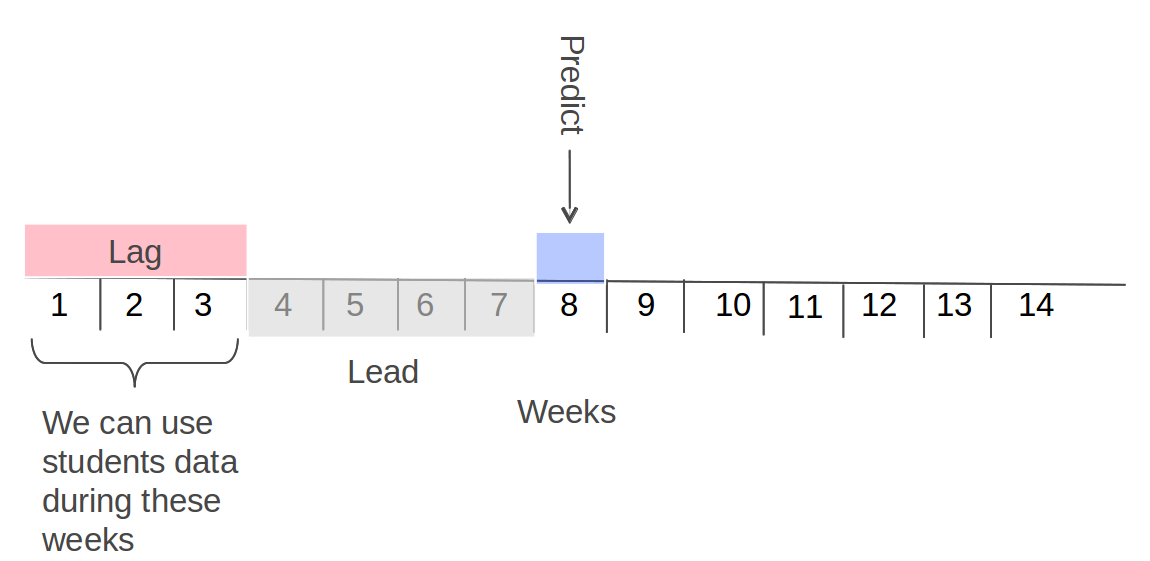
\includegraphics[width=1.0\textwidth]{figures/lead_lag.png}
\end{figure}

\begin{figure}[ht!]
  \caption{Diagram of the flattening process. In this case two weeks of data is used to predict week 13. This prediction problem corresponds to a lead of 11, and a lag of 2.}\label{fig:flattening}
  \centering
    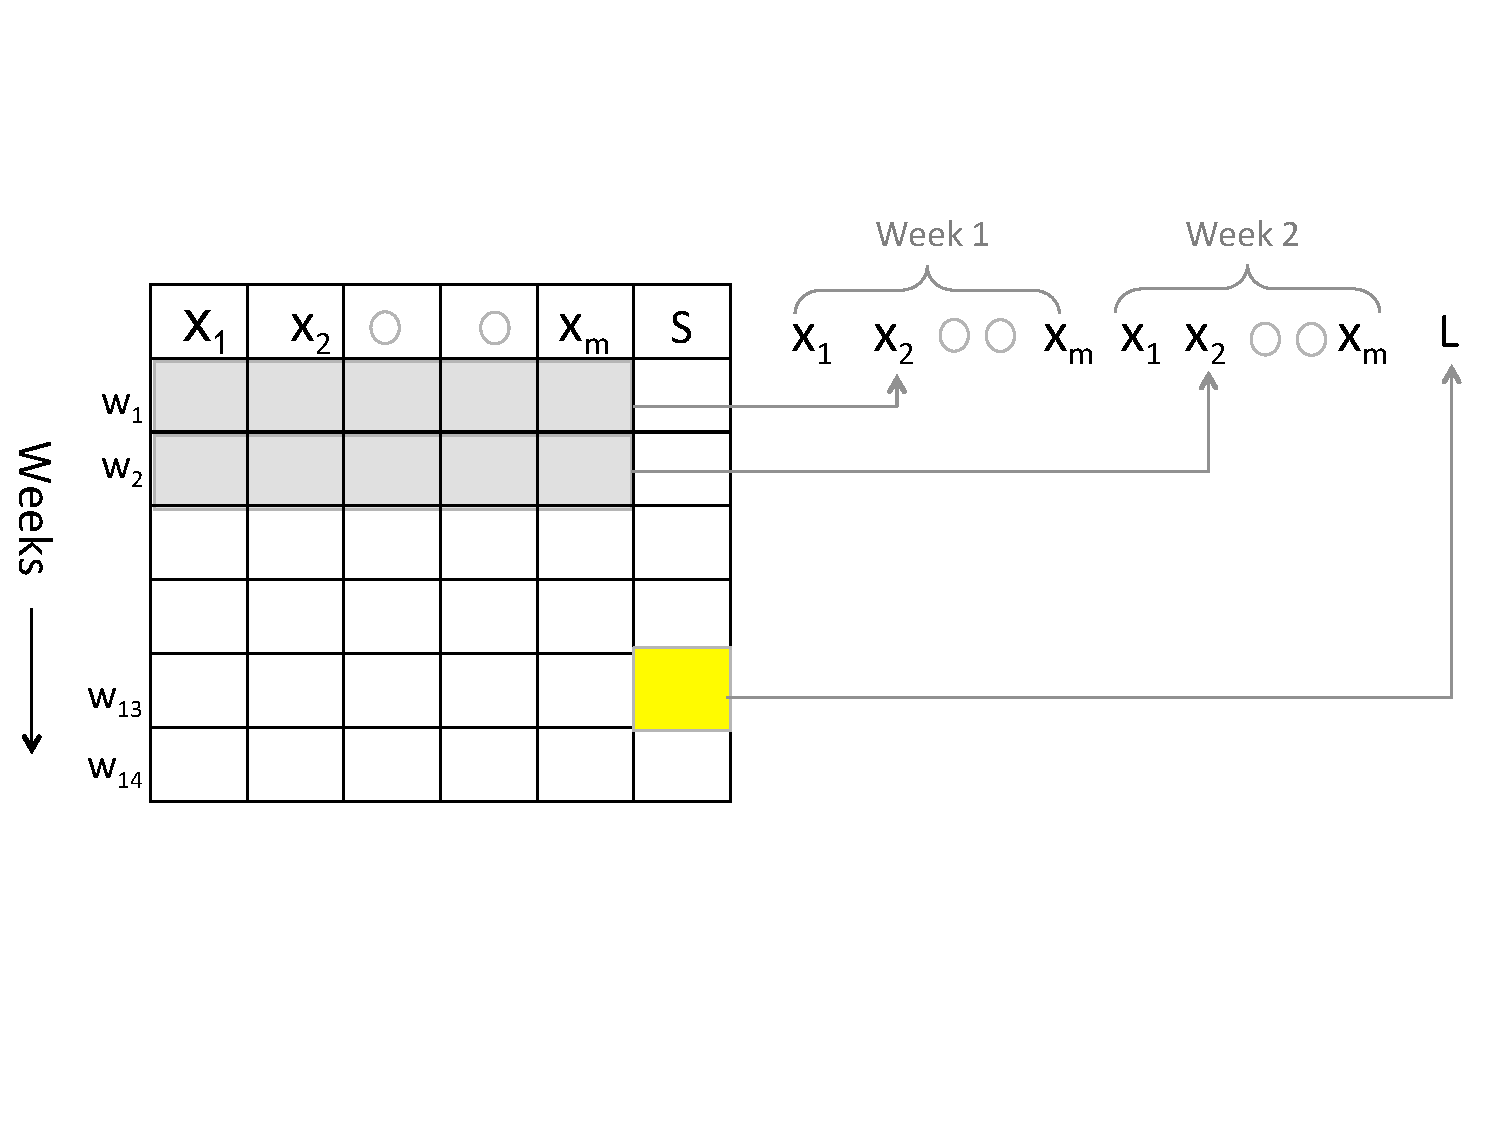
\includegraphics[width=0.7\textwidth]{figures/Flattening}
\end{figure}

\paragraph{Multiple prediction problems}\label{para:multiple_prediction}
Under this definition 91 individual prediction problems exist. For any given week $i$ there are $14-i$ number of prediction problems. Each prediction problem becomes an independent modeling problem which requires a discriminative model. To build discriminative models we utilize a common approach of flattening out the data, that is forming the \cov for the discriminative model by assembling the features from different student-weeks as separate variables. This process is shown in Figure~\ref{fig:flattening}. The example uses data from weeks 1 and 2 (lag of 2) and attempts to predict the \sti for week 13 (lead of 11). 

In this chapter, we present a logistic regression method for building several predictive models. In each of the following sections, we present a model, its advantages and how it is learned. Furthermore, we present a logistic regression variant called randomized logistic regression which we employ to identify feature importance. In Chapter~\ref{chap:delphi} we present results from numerous other approaches for discriminative modeling. 

\section{Logistic Regression}
Logistic regression is a commonly used binary predictive model. It calculates a weighted average of a set of variables, submitted as \cov, as an input to the \textit{logit} function. Thus, the input to the \textit{logit} function, z, takes the following form:
\begin{equation}
 z = \beta_0 + \beta_1 * x_1 + \beta_2 * x_2 + ... \beta_m * x_m  %note N is always reserved for the total number of examples 
 \end{equation}
Here, $\beta_1$ to $\beta_m$ are the coefficients for the feature values, $x_1$ to $x_m$. $\beta_0$ is a constant. The \textit{logit} function, given by, 
\begin{equation}\label{eq:logit}
 y = \frac{1}{1 + e ^{-z}}
 \end{equation}
takes the shape as shown in figure \ref{fig:logit}. Note that the function's range is between 0 and 1, which is optimal for probability. Also note that it tends to `smooth out' at extreme input value, as the range is capped. 

\begin{figure}[ht!]
  \caption{The logit (aka logistic or sigmoid) function. The logit equation is $ y = \frac{1}{1 + e ^{-x}}$. The range of the function is between 0 and 1.}\label{fig:logit}
  \centering
    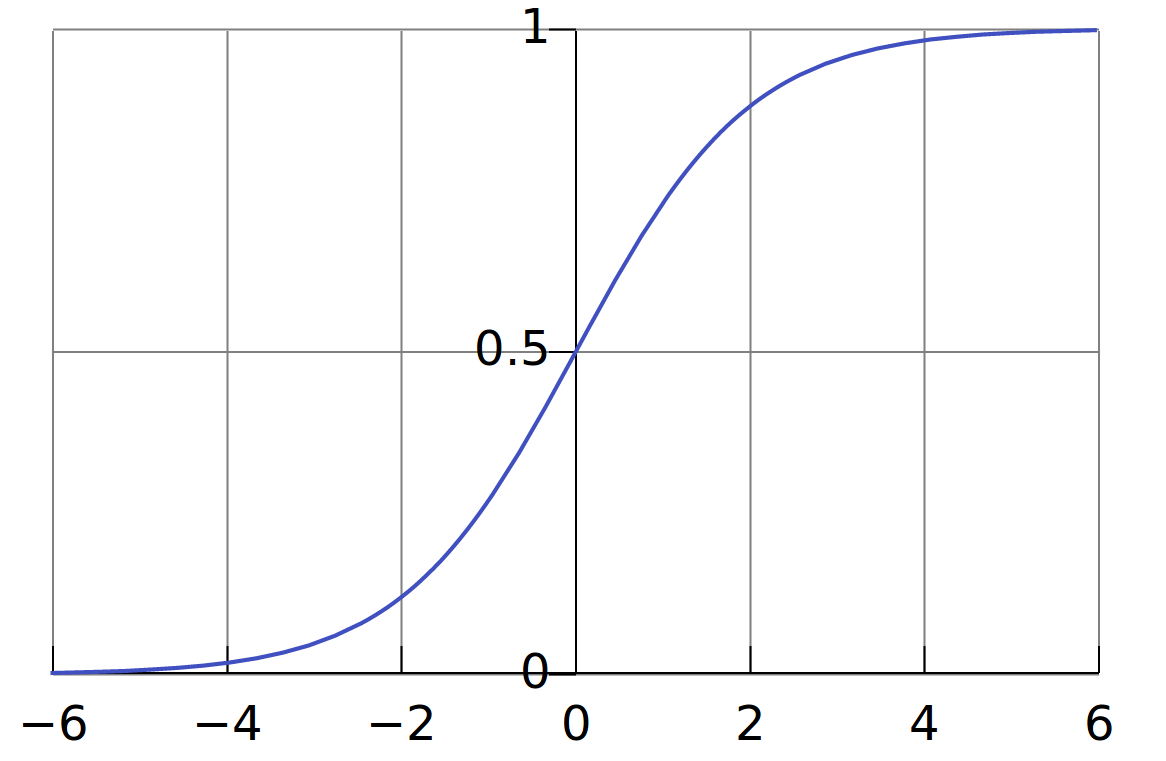
\includegraphics[width=0.7\textwidth]{figures/logit.png}
\end{figure}

For a binary classification problem, such as ours, the output of the \textit{logit} function becomes the estimated probability of a positive training example. These feature weights, or coefficients, are similar to the coefficients in linear regression. The difference is that the output ranges between 0 and 1 due to the logit function, rather than an arbitrary range for linear regression.

\subsection{Learning}
The objective of training a logistic regression model is to find a set of coefficients well suited to fit the data. For the binary classification problem,  as noted before, training involves passing a set of \cov and a corresponding binary label associated with the \cov. After training a model, the predicted probability, or the output of the \textit{logit} function, should predict higher probabilities for the positive `+1' class examples in the training data and a lower probability for the negative `0' class examples. 

There is no closed form solution to find the optimal coefficients to best fit the training data. As a result, training is usually done iteratively through a technique called maximum likelihood estimation \cite{menard2002applied}. First, a random set of coefficients are chosen. At each iteration, an algorithm such as Newton's method is used to find the gradient between what the coefficients predict and what they should predict, and updates the weights accordingly. The process repeats until the change in the coefficients is sufficiently small. This is called convergence. After running this iterative process over all of the training examples, the coefficients represent the final trained model.

\subsection{Inference and evaluation}
With training in place, the next step is evaluating the classifier's performance. A testing set comprised of untrained \cov and labels evaluates the performance of the model on the test data following the steps below: 
\begin{description}\label{steps}
\item {Step 1:} The logistic function learned and presented in ~\ref{eq:logit} is applied to each data point and the estimated probability of a positive label $y_i$ is produced for each.

\item {Step 2:}  A decision rule is applied to determine the class label for each probability estimate $y_i$. The decision rule is given by: 
\begin{equation}\label{eq:decRule}
\hat {L_i} = \left\{ 1, \ if \ y_i \geq \lambda \atop 0, \ if \ y_i < \lambda \right\}
\end{equation}
Given the estimated labels for each data point $\hat{L_i}$ and the true labels $L_i$ we can calculate the confusion matrix, true positives and false positives and thus obtain an operating point on the ROC curve. 
\item {Step 3:} By varying the threshold $\lambda$ in \ref{eq:decRule} the decision rule above we can evaluate multiple points on the ROC curve. We then evaluate the area under the curve and report that as the performance of the classifier on the test data.
\end{description}

\begin{paragraph}
{Predictive accuracy heat map} To present the results for multiple prediction problems for different weeks simultaneously, as discussed in Section~\ref{para:multiple_prediction},  we assemble a heat map of a lower right triangular matrix as shown in Figure~\ref{fig:logistic_regression_heatmap_no_collab2}. The number on the x-axis is the week for which predictions are made of that experiment. The y-axis represents the \lag, or the number of weeks of data used to predict. The color represents the area under the curve for the ROC that the model achieved. Note that as the predicted week increases for a given \lag, it is harder to predict. Likewise, as we increase the \lag for a given prediction week, the stopout value becomes easier to predict. This implies that using more historical information enables a better prediction.
\end{paragraph}

\begin{figure}[!ht]
  \caption{Example heatmap for a logistic regression problem. The heatmap shows how the ROC AUC varied as \lag changed as the target prediction week changed.}\label{fig:logistic_regression_heatmap_no_collab2}
  \centering
    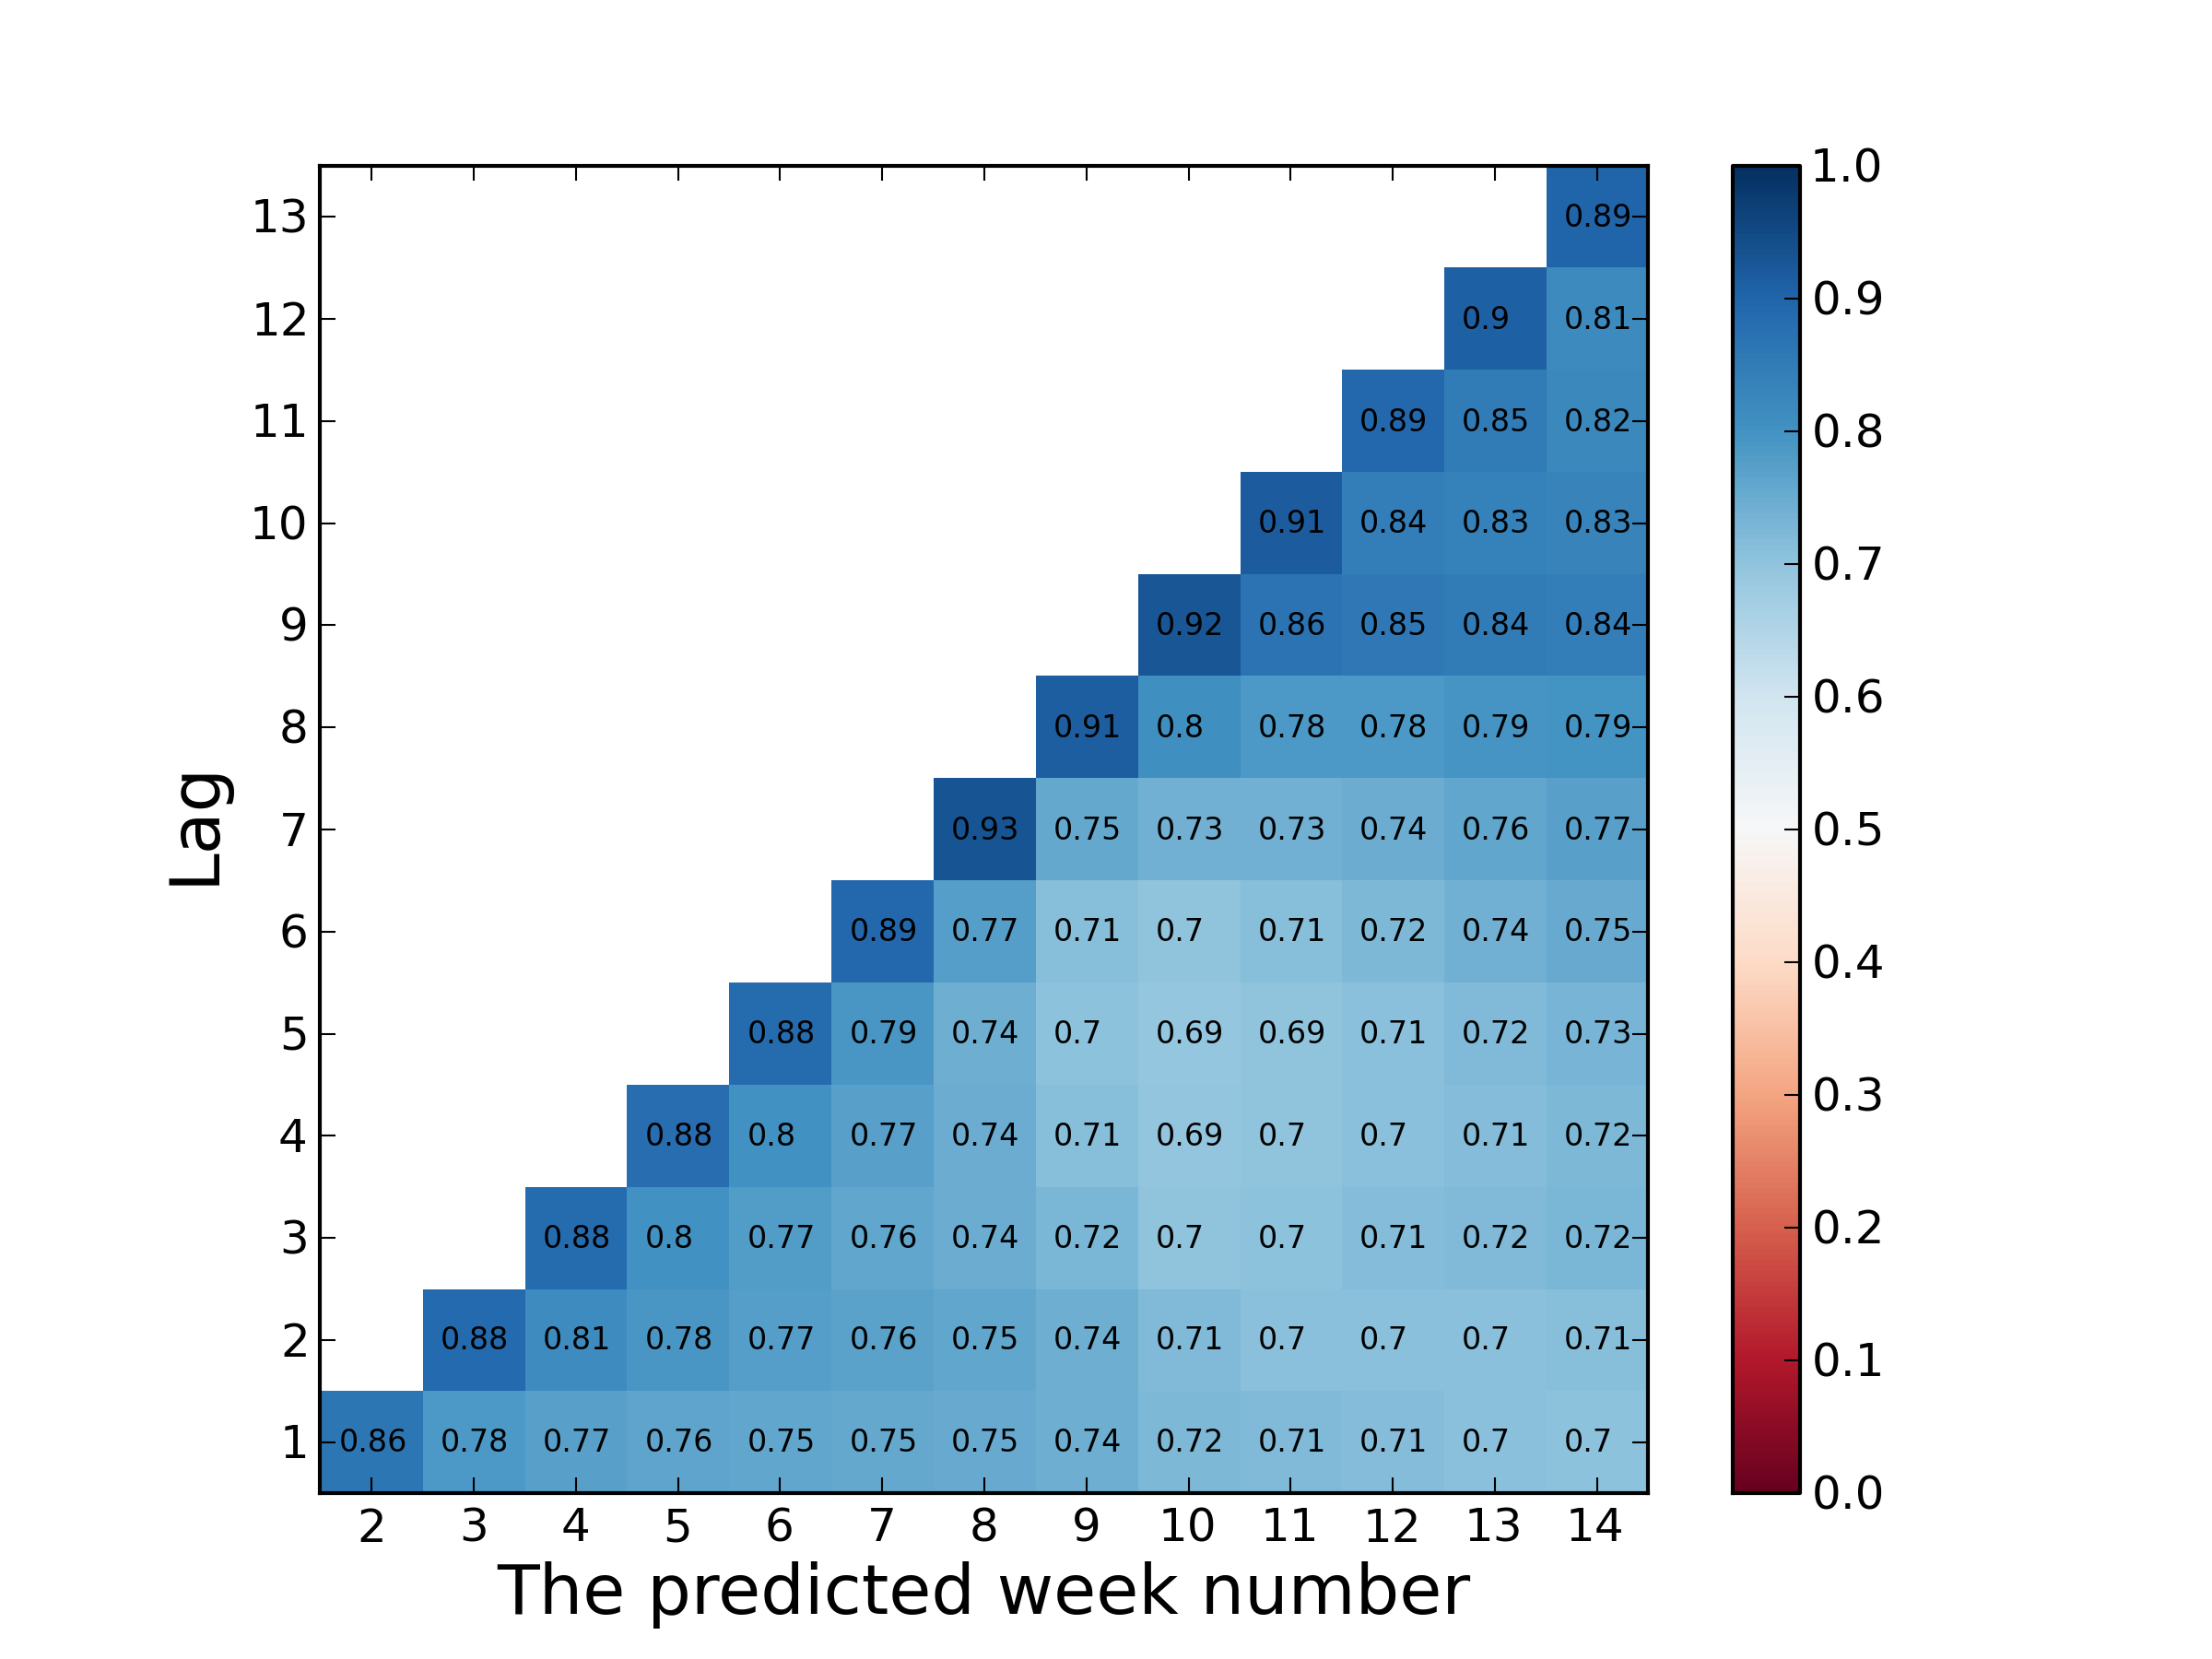
\includegraphics[width=0.8\textwidth]{figures/logreg/no_collab.png}
\end{figure}

\subsection{Attractive properties of logistic regression} 
\begin{itemize}
\item It is relatively simple to understand. 
\item After a model is trained, it provides feature weights, which are useful in assessing the predictive power of features (this will be discussed further in our treatment of the randomized logistic regression model). 
\item It is fast to run. On a single i-7 core machine, for example, running each of the 91 prediction problems on all 4 cohorts took ~25 hours.
\end{itemize}

\section{Predicting stopout with logistic regression}
We applied logistic regression to student persistence prediction. We used the 27 interpretive features as described in Chapter~\ref{chap:features} to form the feature vectors, and maintained the \sti value as the label. We used the features themselves, rather than the PCA features so as to analyze predictor importance.

\subsection{Experimental setup}
To perform logistic regression analysis, we executed the ensuing steps for every lead, \lag and cohort combination
\footnote{
We used the logistic regression implementation of an open source machine learning library, called scikit-learn. We chose this library because it is well known and tested, fast (the core maximum likelihood estimation algorithm is written in C), with an easy to use python interface. In addition, the scikit-learn library includes an easy interface for cross validation and feature normalization.}:
\begin{enumerate}
\item Performed 10 fold cross validation on the training set. As outlined in the evaluation chapter, this involved training the model on 9 folds of the train dataset and testing on the last fold.
\item Trained a logistic regression model on the entire train dataset.
\item Applied the model to the test dataset by putting each data point through the model then applying the decision rule in ~\ref{eq:decRule} and following the steps in ~\ref{steps} to determine the AUC under the ROC.
%the resulting probability of \sti versus the truth \sti label.
\item Evaluating the model using mean cross validation ROC AUC and test set ROC AUC.
\end{enumerate}

\subsection{Experimental results}
Figures \ref{fig:logistic_regression_heatmap_no_collab} through \ref{fig:logistic_regression_heatmap_wiki_only} summarize the AUC of the receiver operating characteristic for all four cohorts over each lead and \lag combination. Overall, logistic regression predicted dropout with very high accuracy. Some experiments, such as a \lag of 7, predicting week 8 in the \both cohort achieved accuracies as high as 0.95, a fantastic result (Figure \ref{fig:logistic_regression_heatmap_forum_and_wiki}). Moreover, the entire diagonal of the \neither cohort's heatmap (Figure \ref{fig:logistic_regression_heatmap_no_collab}) resulted in an AUC greater than 0.88. This diagonal represents experiments with a lead of one. Thus, we can surmise that the extracted features are highly capable of predicting stopout, especially when the prediction week is fairly near the \lag week.

Across all experiments, the predictive models of the \neither cohort achieved the highest predictive accuracies. This is because \neither is by far the largest cohort, which resulted in high performing, stable accuracy for all 91 experiments. Conversely, the \wiki cohort performed terribly for many experiments. In fact, for some \lag and predicted week combinations, the model could not even compute an AUC because there were not enough examples to test on.

\begin{figure}[ht!]
  \caption{Logistic regression results for the \neither cohort.}\label{fig:logistic_regression_heatmap_no_collab}
  \centering
    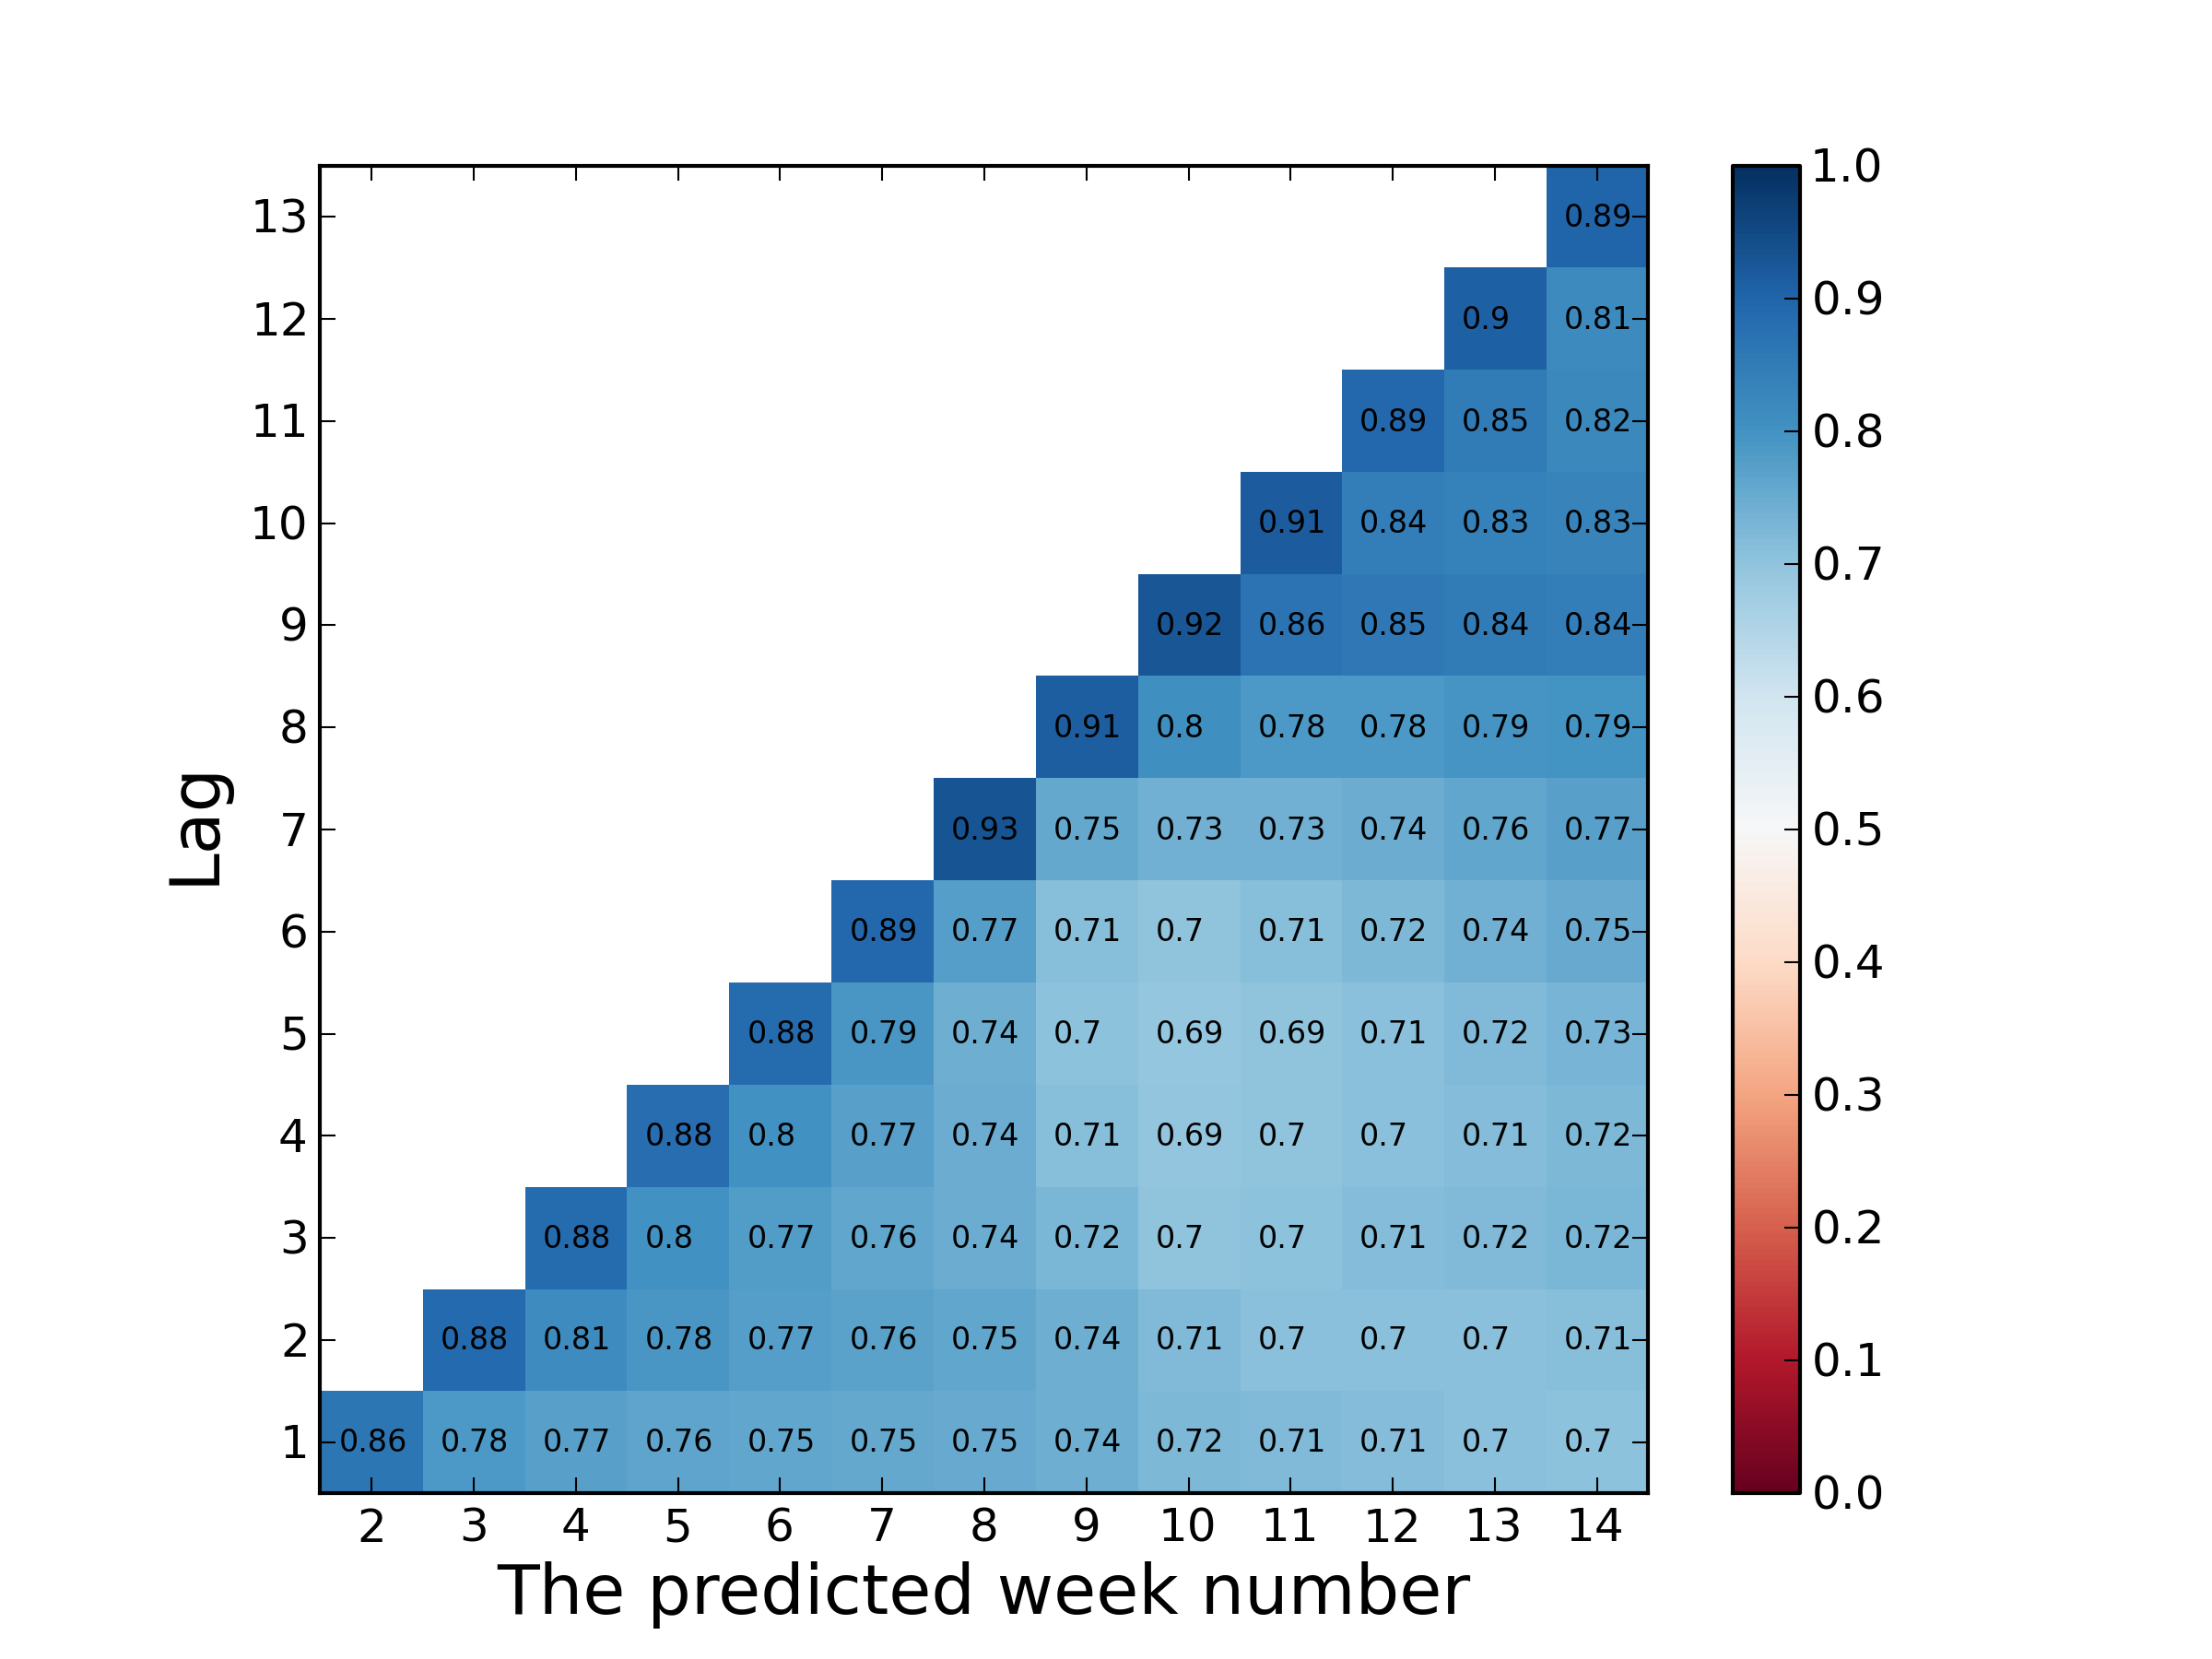
\includegraphics[width=1.0\textwidth]{figures/logreg/no_collab.png}
\end{figure}

\begin{figure}[ht!]
  \caption{Logistic regression results for the \forum cohort.}\label{fig:logistic_regression_heatmap_forum_only}
  \centering
    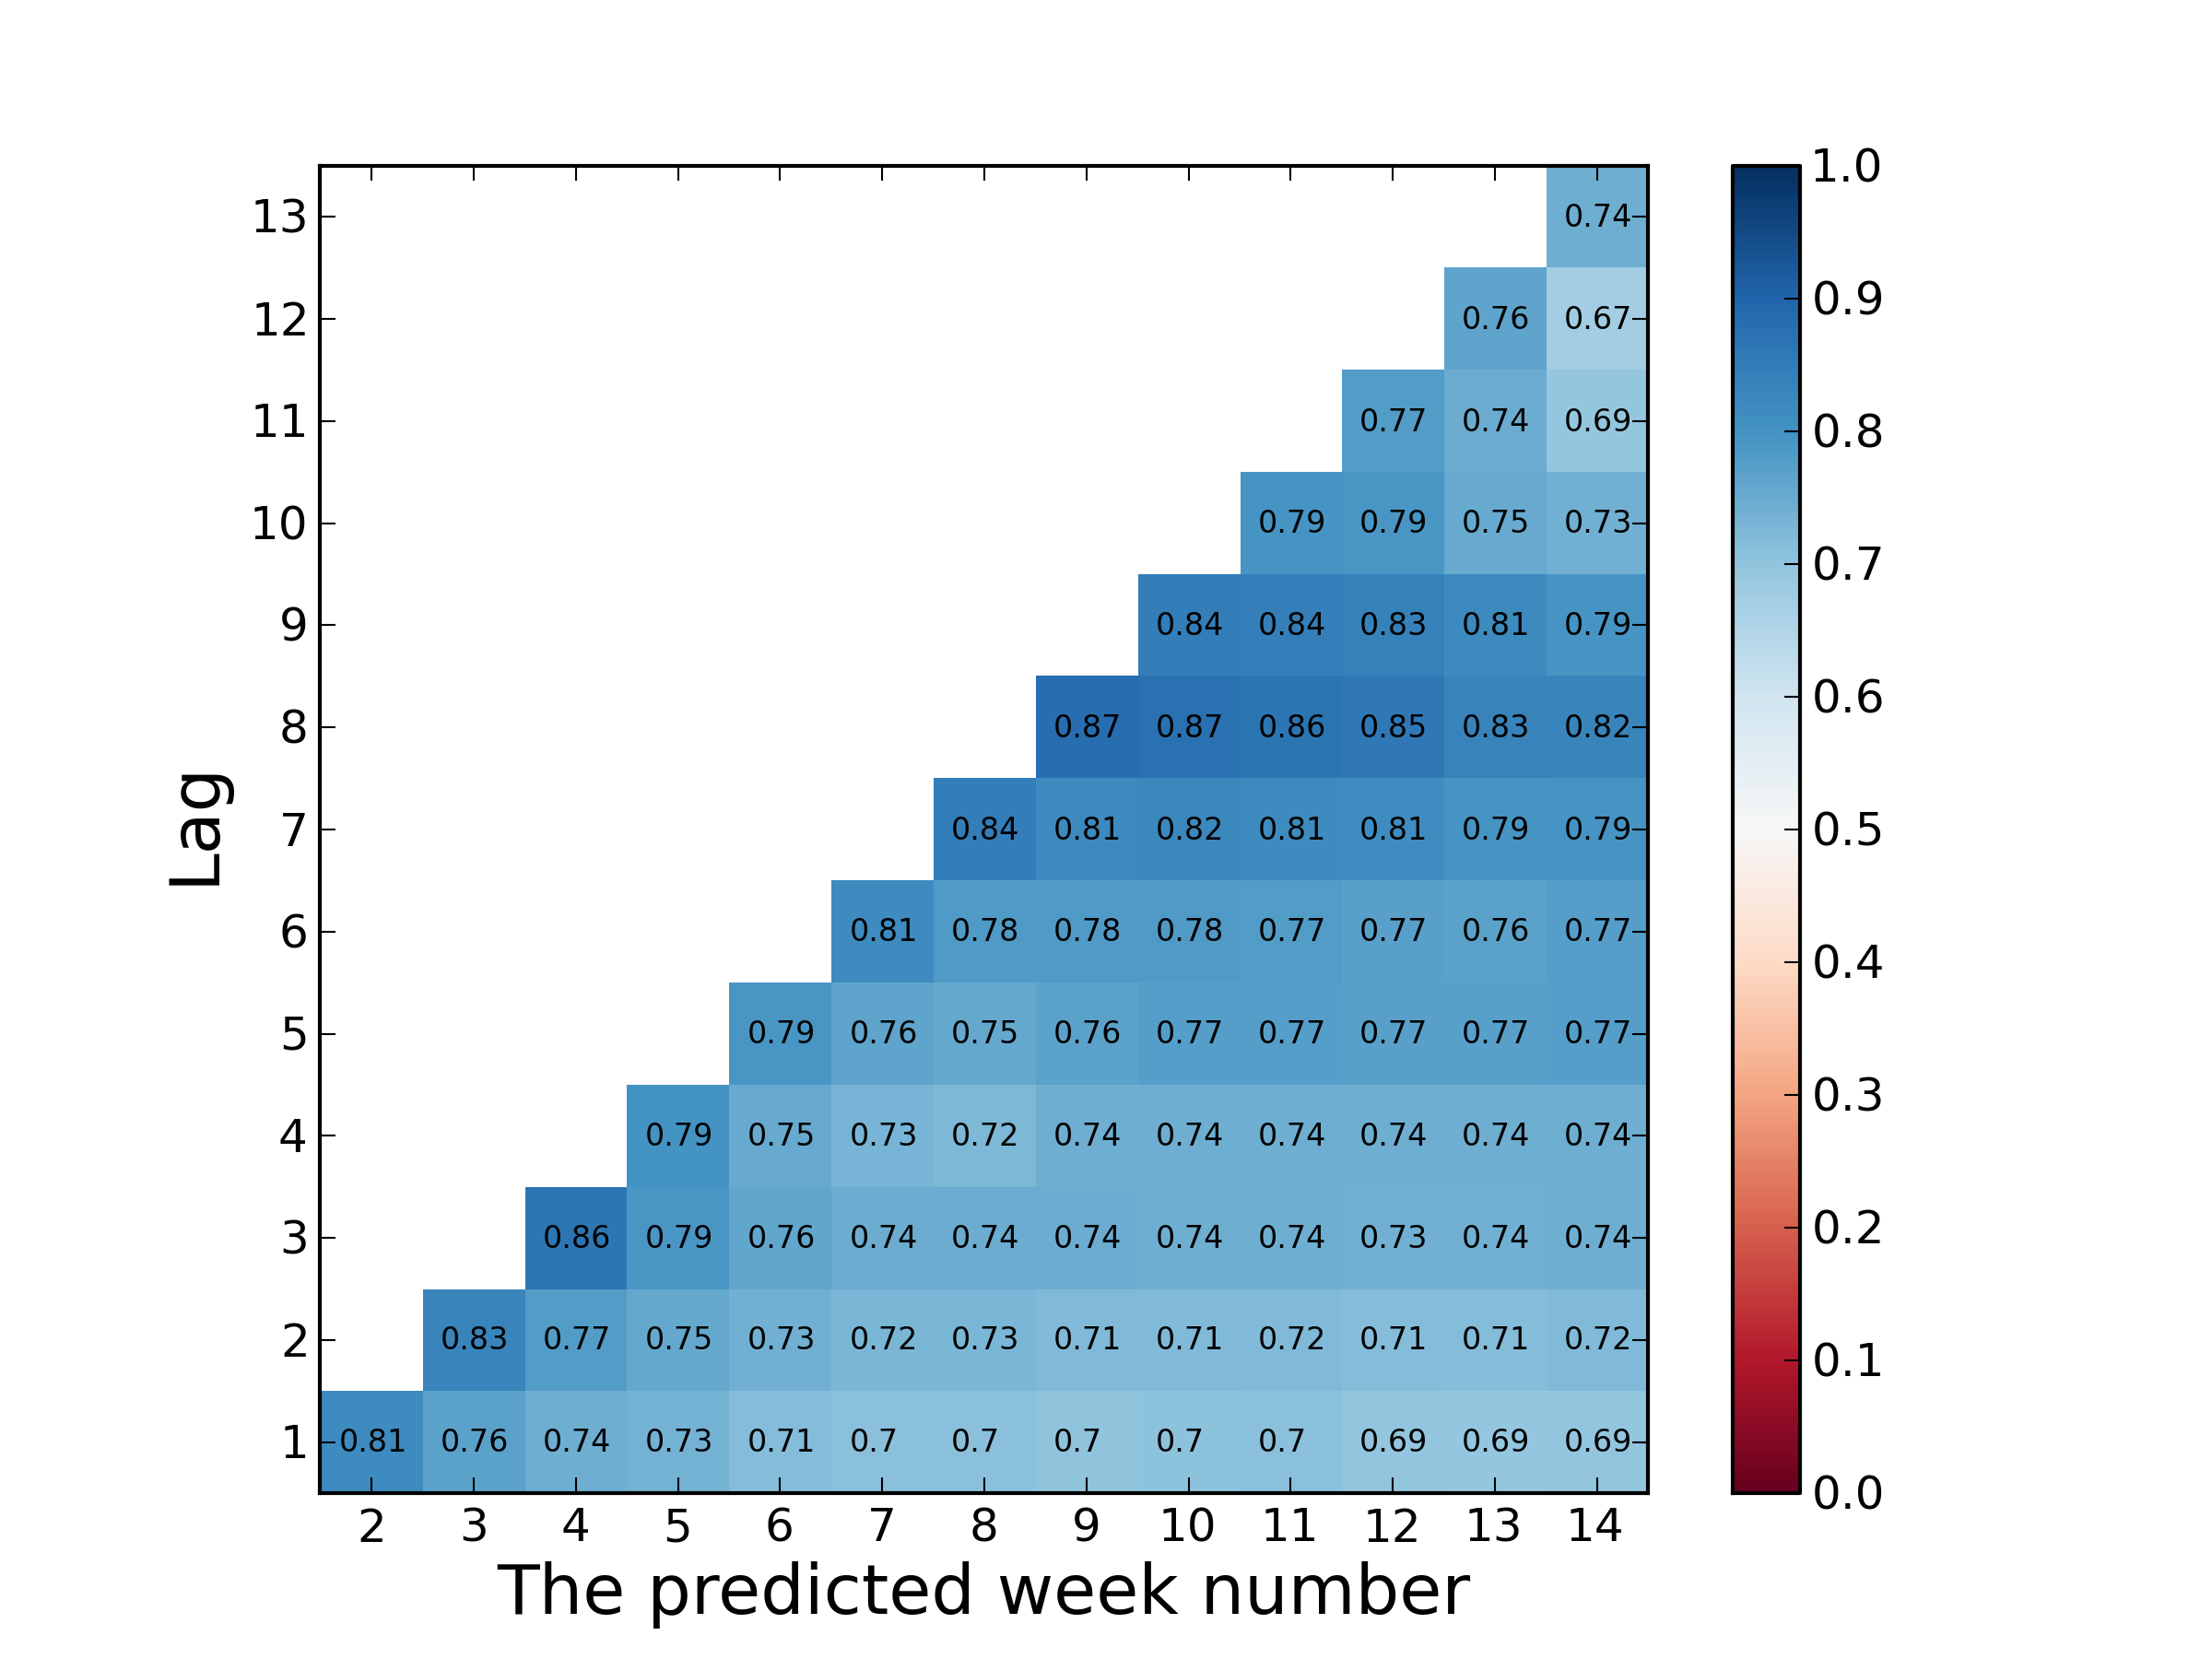
\includegraphics[width=1.0\textwidth]{figures/logreg/forum_only.png}
\end{figure}

\begin{figure}[ht!]
  \caption{Logistic regression results for the \both cohort.}\label{fig:logistic_regression_heatmap_forum_and_wiki}
  \centering
    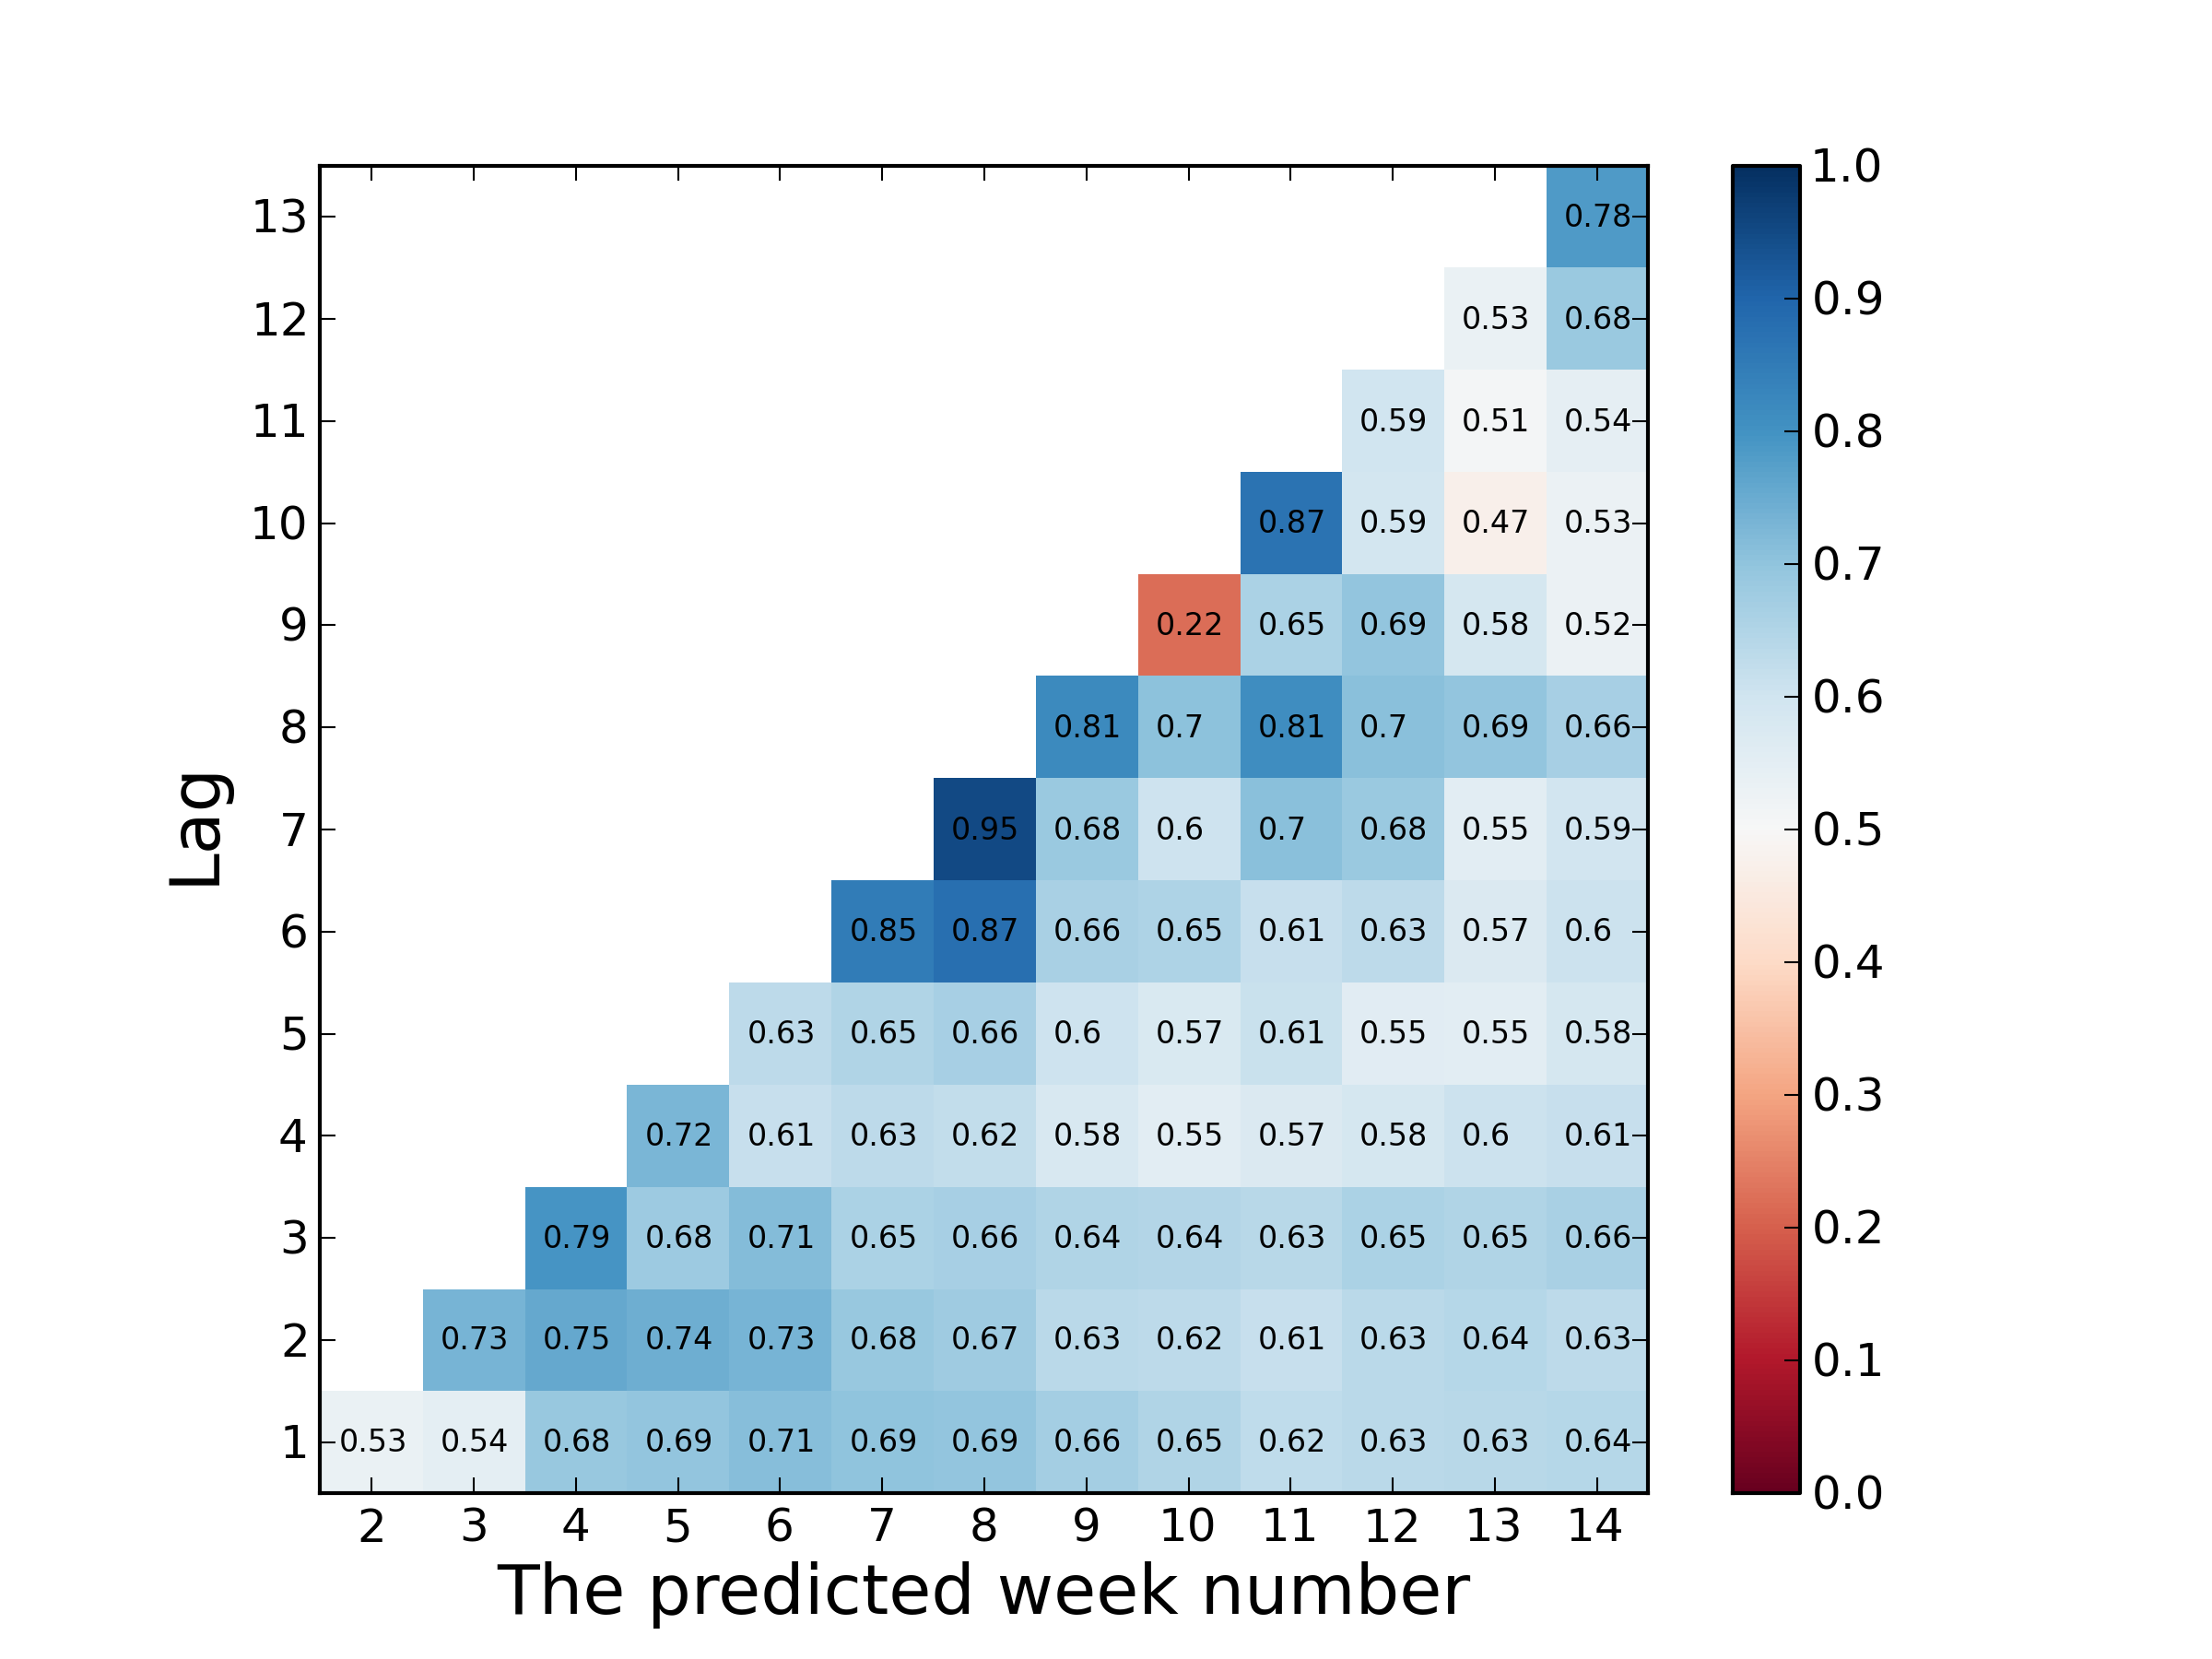
\includegraphics[width=1.0\textwidth]{figures/logreg/forum_and_wiki.png}
\end{figure}

\begin{figure}[ht!]
  \caption{Logistic regression results for the \wiki cohort.}\label{fig:logistic_regression_heatmap_wiki_only}
  \centering
    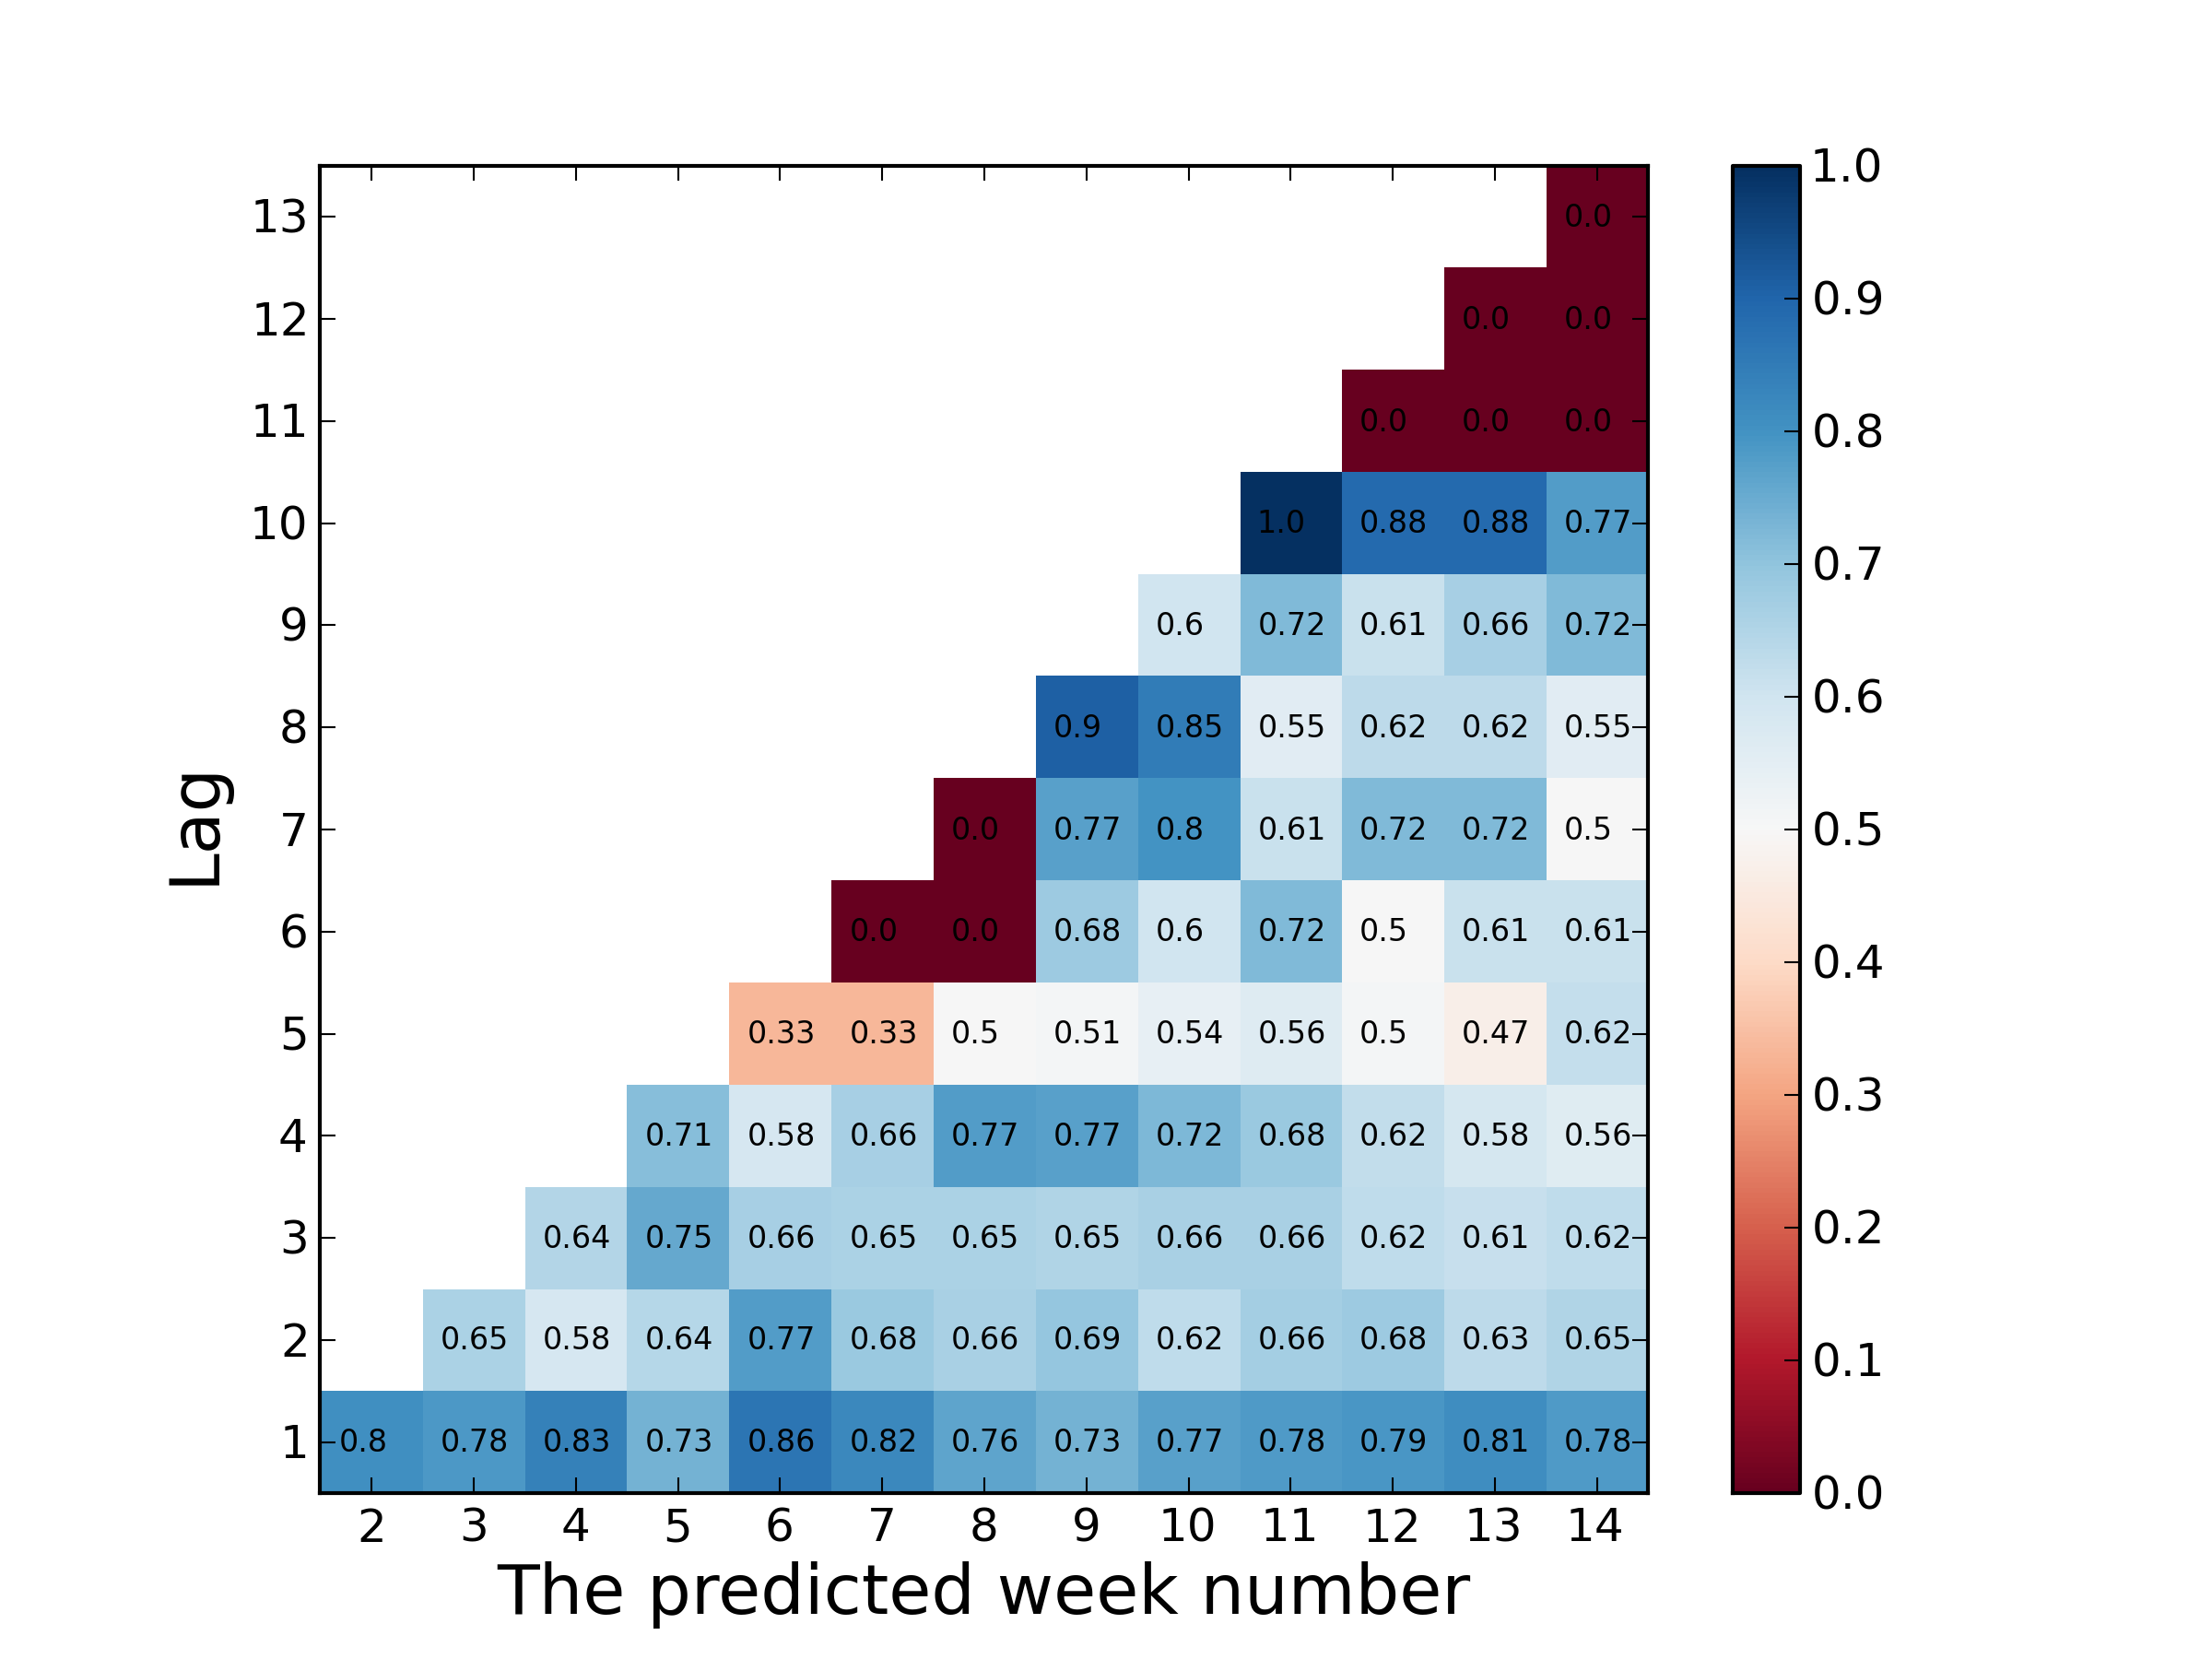
\includegraphics[width=1.0\textwidth]{figures/logreg/wiki_only.png}
\end{figure}

What follows is a deeper explanation of two interesting prediction problems and their results.

\paragraph{Are there early signs of stopout?}
One extremely interesting prediction problem is trying to predict student persistence into the last week of the course using a single week of data. Practically speaking, this would enable platform providers and instructors to predict which students would finish the course by the end of the first week. Potentially, this would allow instructors to interpret the reason for student stopout as motivational (such as just browsing) rather than course-specific reasons (such as the content becoming too difficult), because the students have not been exposed to much content yet. Furthermore, early-sign stopout prediction could allow courses to target certain types of students for some type of intervention or special content. If our models are successful, the results would imply that our extracted features are capturing a student's persistence far in advance. Remarkably across cohorts, the generated models achieved an AUC of at least 0.64, and reached as high as 0.78 in the case of the \wiki cohort. 

The \wiki AUC of 0.78, or even the \neither of 0.7 suggests it is possible to roughly estimate which students will finish the course. Implications include the ability to reach out to students likely to stop the course before they become disengaged, or giving a professor a rough indication of how many students to expect each week. If these predictions hold true for other courses, a prediction model could be used to measure the success of course experiments, such as changing course content.

In the case of the \wiki cohort, the model performed well for most later predictive weeks given a \lag of one. This indicates two things. Firstly, \wiki students show remarkably high early signs of persistence. Secondly, given more students, predictive models of the \wiki cohort would likely perform well. Owing largely to the small pool size of the \wiki cohort, model performance suffered, especially as \lag increased, because there were not enough students to appropriately train on. However, with a lead of one, the models used more student's data because we included all students who started in the course.

\paragraph{The prediction spike after the midterm}
Leading up to the midterm (in week 8), making predictions using a \lag of $i$, where $i$ is the current week, yields a fairly consistent AUC. In other words, students who will \sti after the midterm resemble their persistent counterparts up until week 8. However, using \lag 8 instead of 7, thereby including midterm data, produces an upward prediction spike in all four cohorts.

Perhaps the most striking spike example is in the most consistent cohort, the \neither students. If the model attempts to predict using a only lag 7, it realizes an AUC of 0.75. If the model expands to include midterm week data from week 8 and attempts to predict who will be in the course the next week, it achieves an AUC of 0.91! This is a significant spike. Similarly, the \both cohort increases AUC significantly from 0.68 in week 7 to 0.81 in week 8.

With the addition of the midterm week data the model is equipped to make reasonably consistent predictions through the end of the course. In fact, for the two cohorts of significant size, the region including and beyond week 8 achieves the highest AUCs of the entire course. This suggests that the midterm exam is a significant milestone for \sti prediction. It follows that most students who complete the midterm finish the course. For the two smaller cohorts, \wiki and \both, the region beyond week 8 realizes terrible predictive power because too few students remain in the course to accurately train on.

\section{Randomized Logistic Regression}
Another use of logistic regression is to assess the importance of features. Our model analyzes 27 features to model \sti. In order to best fit a training set, the model optimizes weights for each feature (outlined in the logistic regression section). By weighting the features we gain a sense of how predictive each feature is. However, the logistic regression model misses the mark if two variables are highly predictive, yet very correlated, because it will only select one. The unselected feature will appear to have a low coefficient. To work around single feature selection we perform Randomized logistic regression which works as follows: 

\begin{description}
\item {Step 1:} Sample without replacement  75\% of the training data each time. 

\item {Step 2:} Train a logistic regression model on the sub-sampled data (with regularization).

\item {Step 3:} For every feature evaluate $b_s^{i}=\mu(w_i,th)$ where $\mu$ is a unit step function and $w_i$ is the \coeff for \co $i$ and $th$ is the threshold we set to deem the feature important. This is set at 0.25. 

\item {Step 4:} Repeat Steps 1, 2 and 3 a total of 200 times. 

\item {Step 5:} Estimate the importance of the \co $i$ by $\sum_s b_s^{i}$. 

\end{description}

We applied \rLR logistic regression to the \sti prediction problem using the exact same process as we did in logistic regression (e.g. flattening a feature set using lead and \lag values etc.) This technique is also referred to as stability selection \cite{meinshausen2010stability}.


\subsection{Experimental setup}
We ran randomized logistic regression for every lead, \lag and cohort combination. For each experiment, randomized logistic regression resulted in a vector of \cov weights. Each weight ranged from 0 to 1.
\footnote{We used the scikit-learn Randomized Logistic Regression implementation.}

\subsection{Experimental results}
Randomized logistic regression analysis gave us fascinating covariate weight vectors for all 91 experiments and all cohorts. For each experiment the randomized logistic regression gives us weights for all the \cov which are student features for different weeks.  In order to gain a more quantitative grasp of which features matter, as well as which week's data mattered for different prediction problem, we performed two different types of aggregations. 

\begin{paragraph}
{Week invariant feature importance} To calculate the importance of a feature, we first evaluate its importance in each of the 91 experiments. We sum the weights associated with it across different weeks, then divide it with the sum of all weights for that experiment. This gives its weight relative to every other feature in that particular experiment. We illustrate this procedure for evaluating feature 1's importance in an experiment where the lag=3 in Figure~\ref{fig:wif}. After quantifying importance for the feature of each experiment, we average the number to get the week-invariant feature importance.  Figures \ref{fig:randomized_logistic_regression_no_collab} to \ref{fig:randomized_logistic_regression_wiki_only} summarize these normalized average feature weights. 

\begin{figure}[ht!]
  \caption{Aggregating feature 1's weights to assemble relative feature importance for a single experiment. In this example, the lag is 3. Three weeks data is used to predict a \sti in a future week. The Randomized logistic regression gives the weights for all 27 features for all three weeks (unnormalized). To assemble the week invariance relative weight for feature 1 we sum the weights and divide it with the total weights. We note that this is a heuristic. }\label{fig:wif}
  \centering
    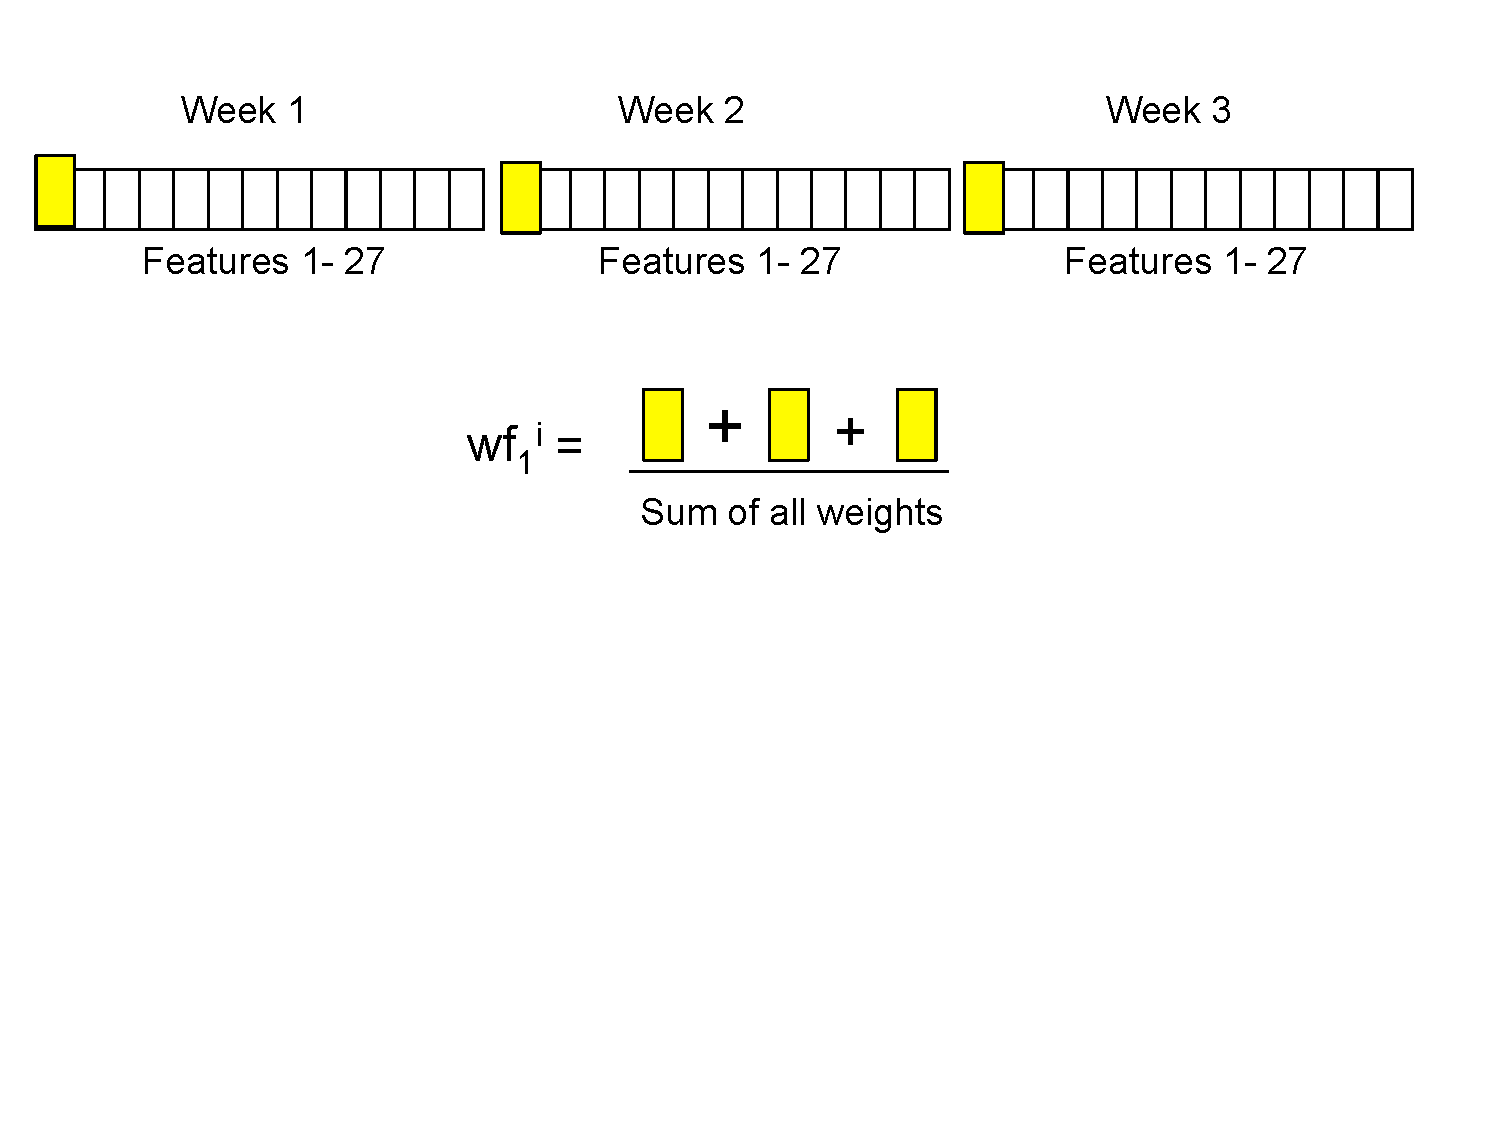
\includegraphics[width=0.6\textwidth]{figures/wif}
\end{figure}

\begin{figure}[ht!]
  \caption{Feature importances for the \neither cohort.}\label{fig:randomized_logistic_regression_no_collab}
  \centering
    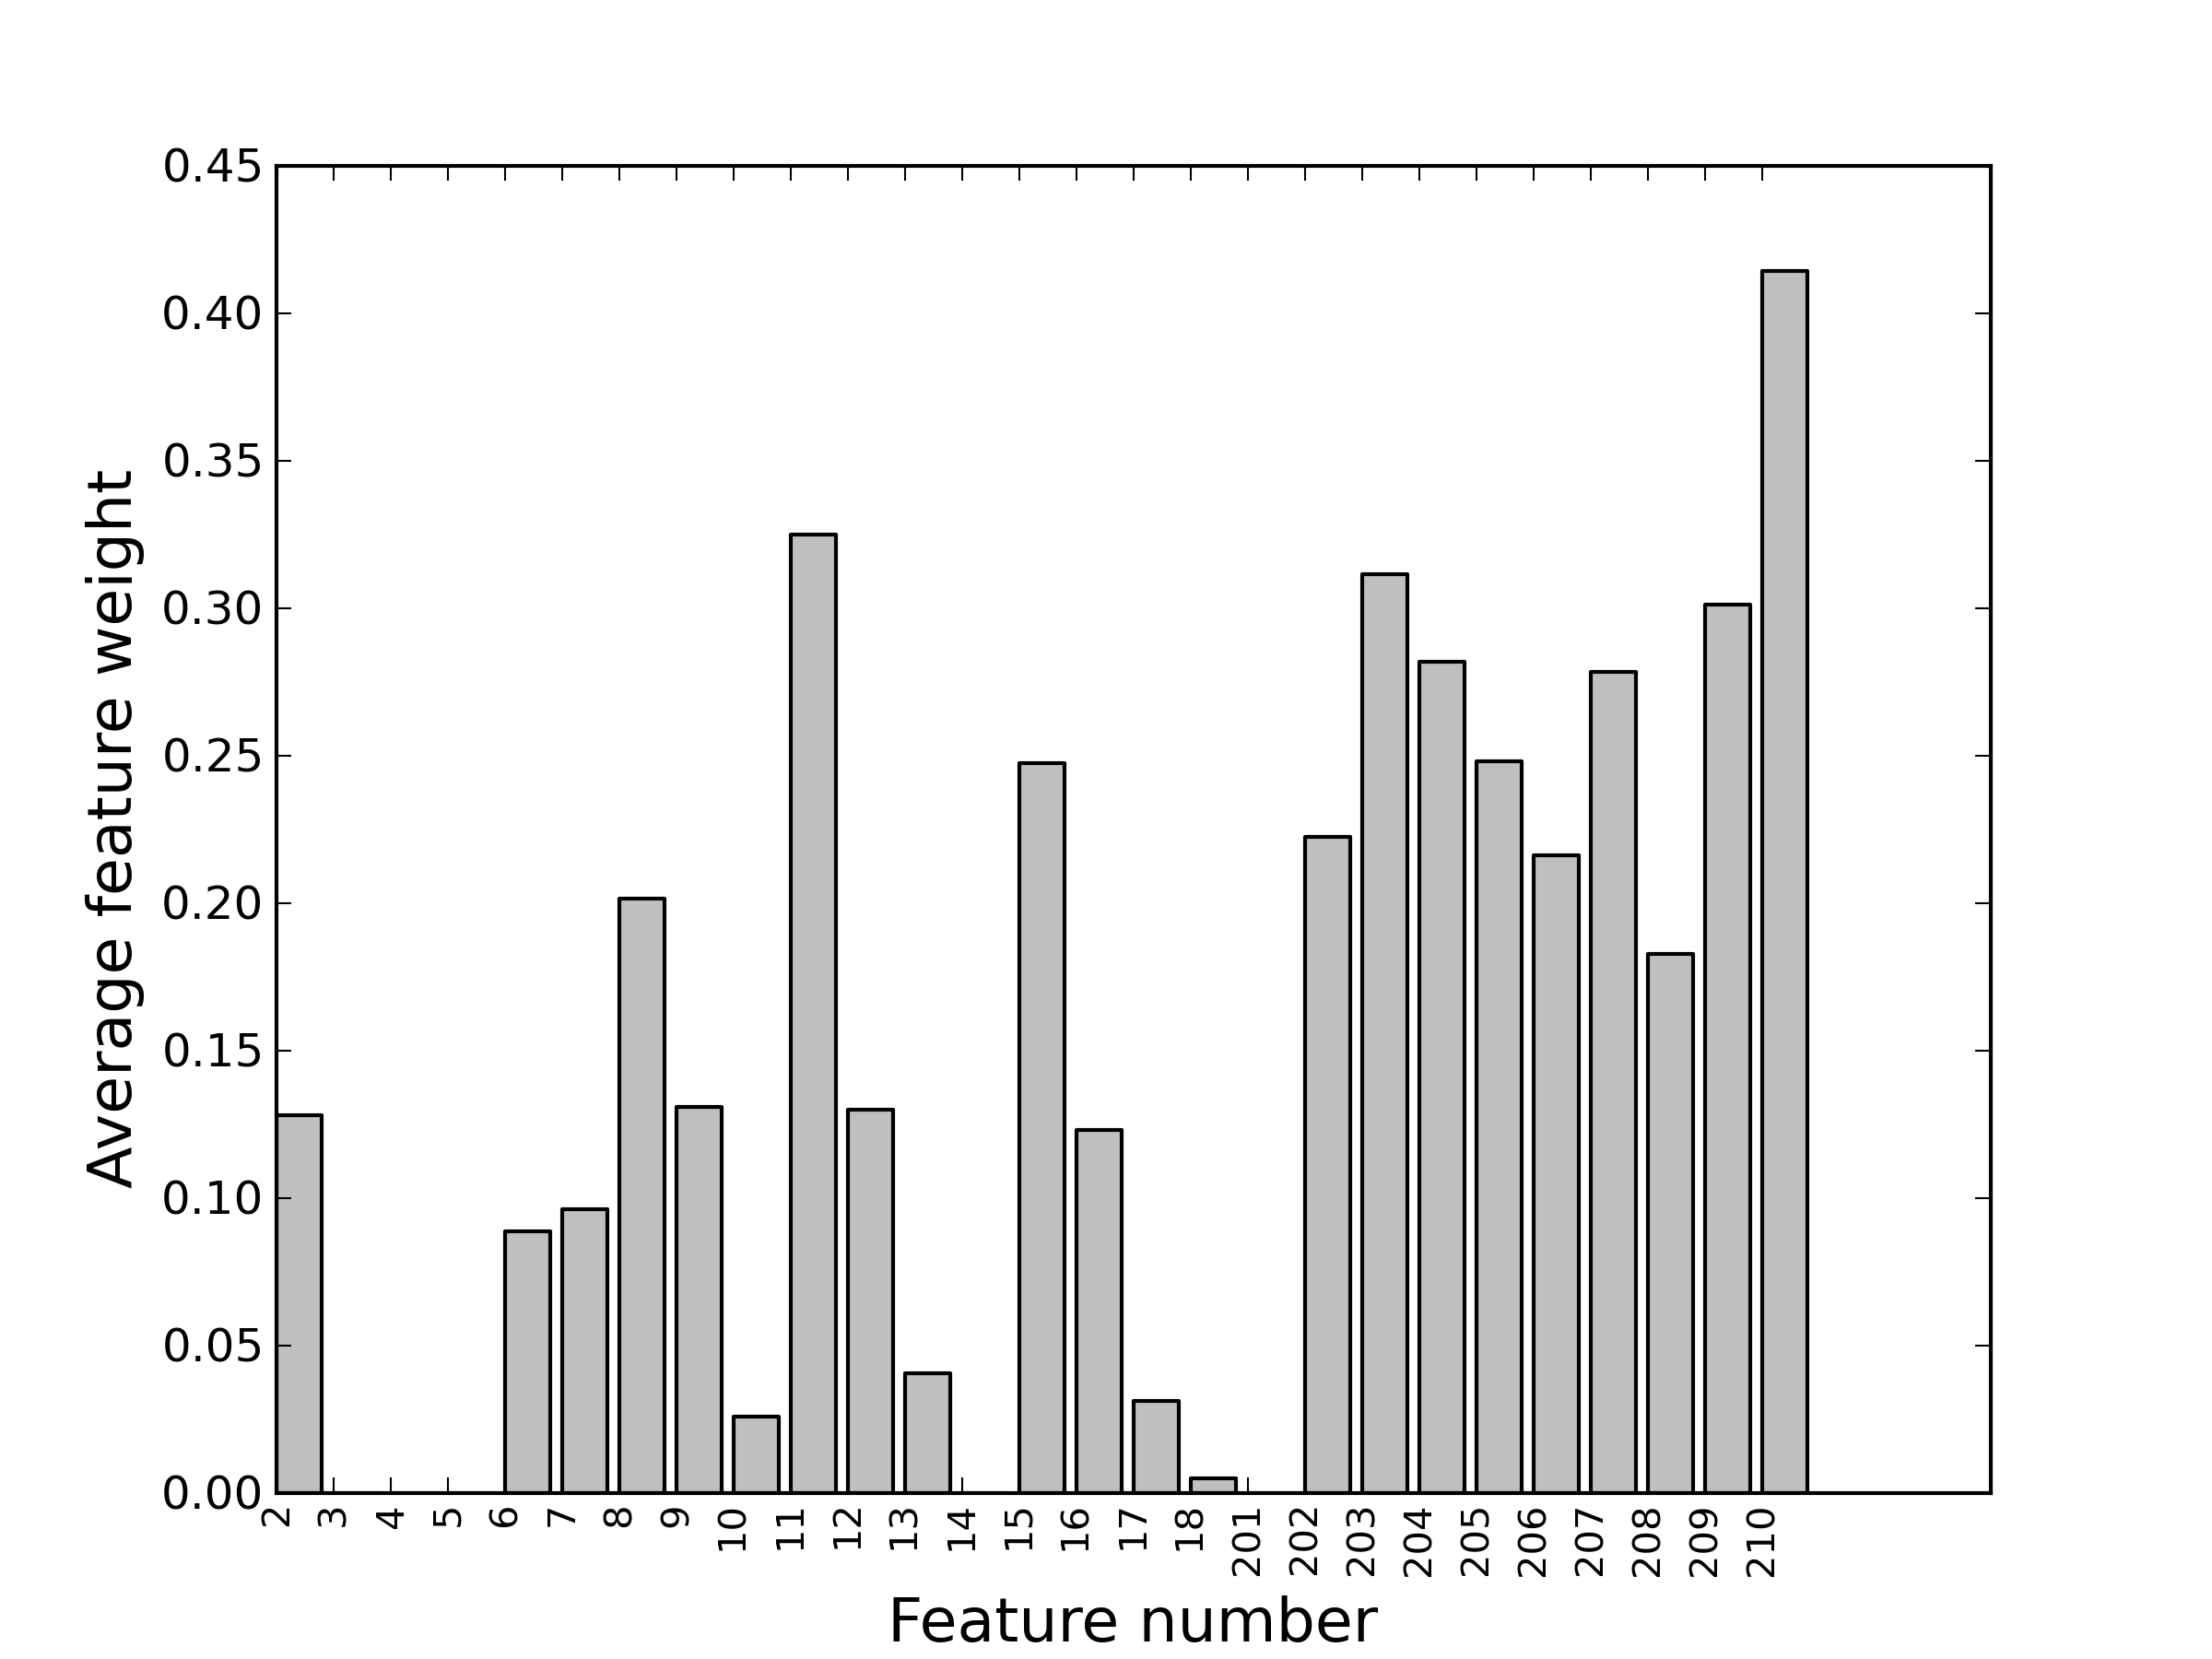
\includegraphics[width=0.7\textwidth]{figures/logreg/randomized_no_collab.png}
\end{figure}

The first thing that struck us as we looked at these plots was the difference in feature weights between the self-proposed features and the crowd-proposed features. In all four cohorts, the majority of the weight lies in the crowd-proposed features \ref{section:crowdself} (\x{201} through \x{210})! Clearly, the crowd can be utilized to a great degree. As features mostly represent high level constructs, such as the percentiles (\x{202} and \x{203}), these plots suggest that those types of features have a very high predictive power. Additionally, they mostly involve the submissions table in MOOCdb. This includes the lab grade (\x{206}), pset grade (\x{207}) and predeadline submission time (\x{210})).

In the \neither cohort, the feature most indicative of \sti is the average predeadline submission time. The \forum cohort looks very similar, but uses a broader spectrum of features. In particular, we see that \x{5}, the average length of forum posts, is also highly predictive (of course, this could not have shown up in the \neither cohort, as by definition those students do not participate in the forum). Interestingly, we see a very low predictive power from the number of forum posts(\x{3}) and the number of forum replies (\x{201}), despite the fact that the length of the forum post is very important. This could imply that longer posts are indicative of more engagement in the course, or a greater mastery of the material.

\begin{figure}[ht!]
  \caption{Feature importances for the \forum cohort.}\label{fig:randomized_logistic_regression_forum_only}
  \centering
    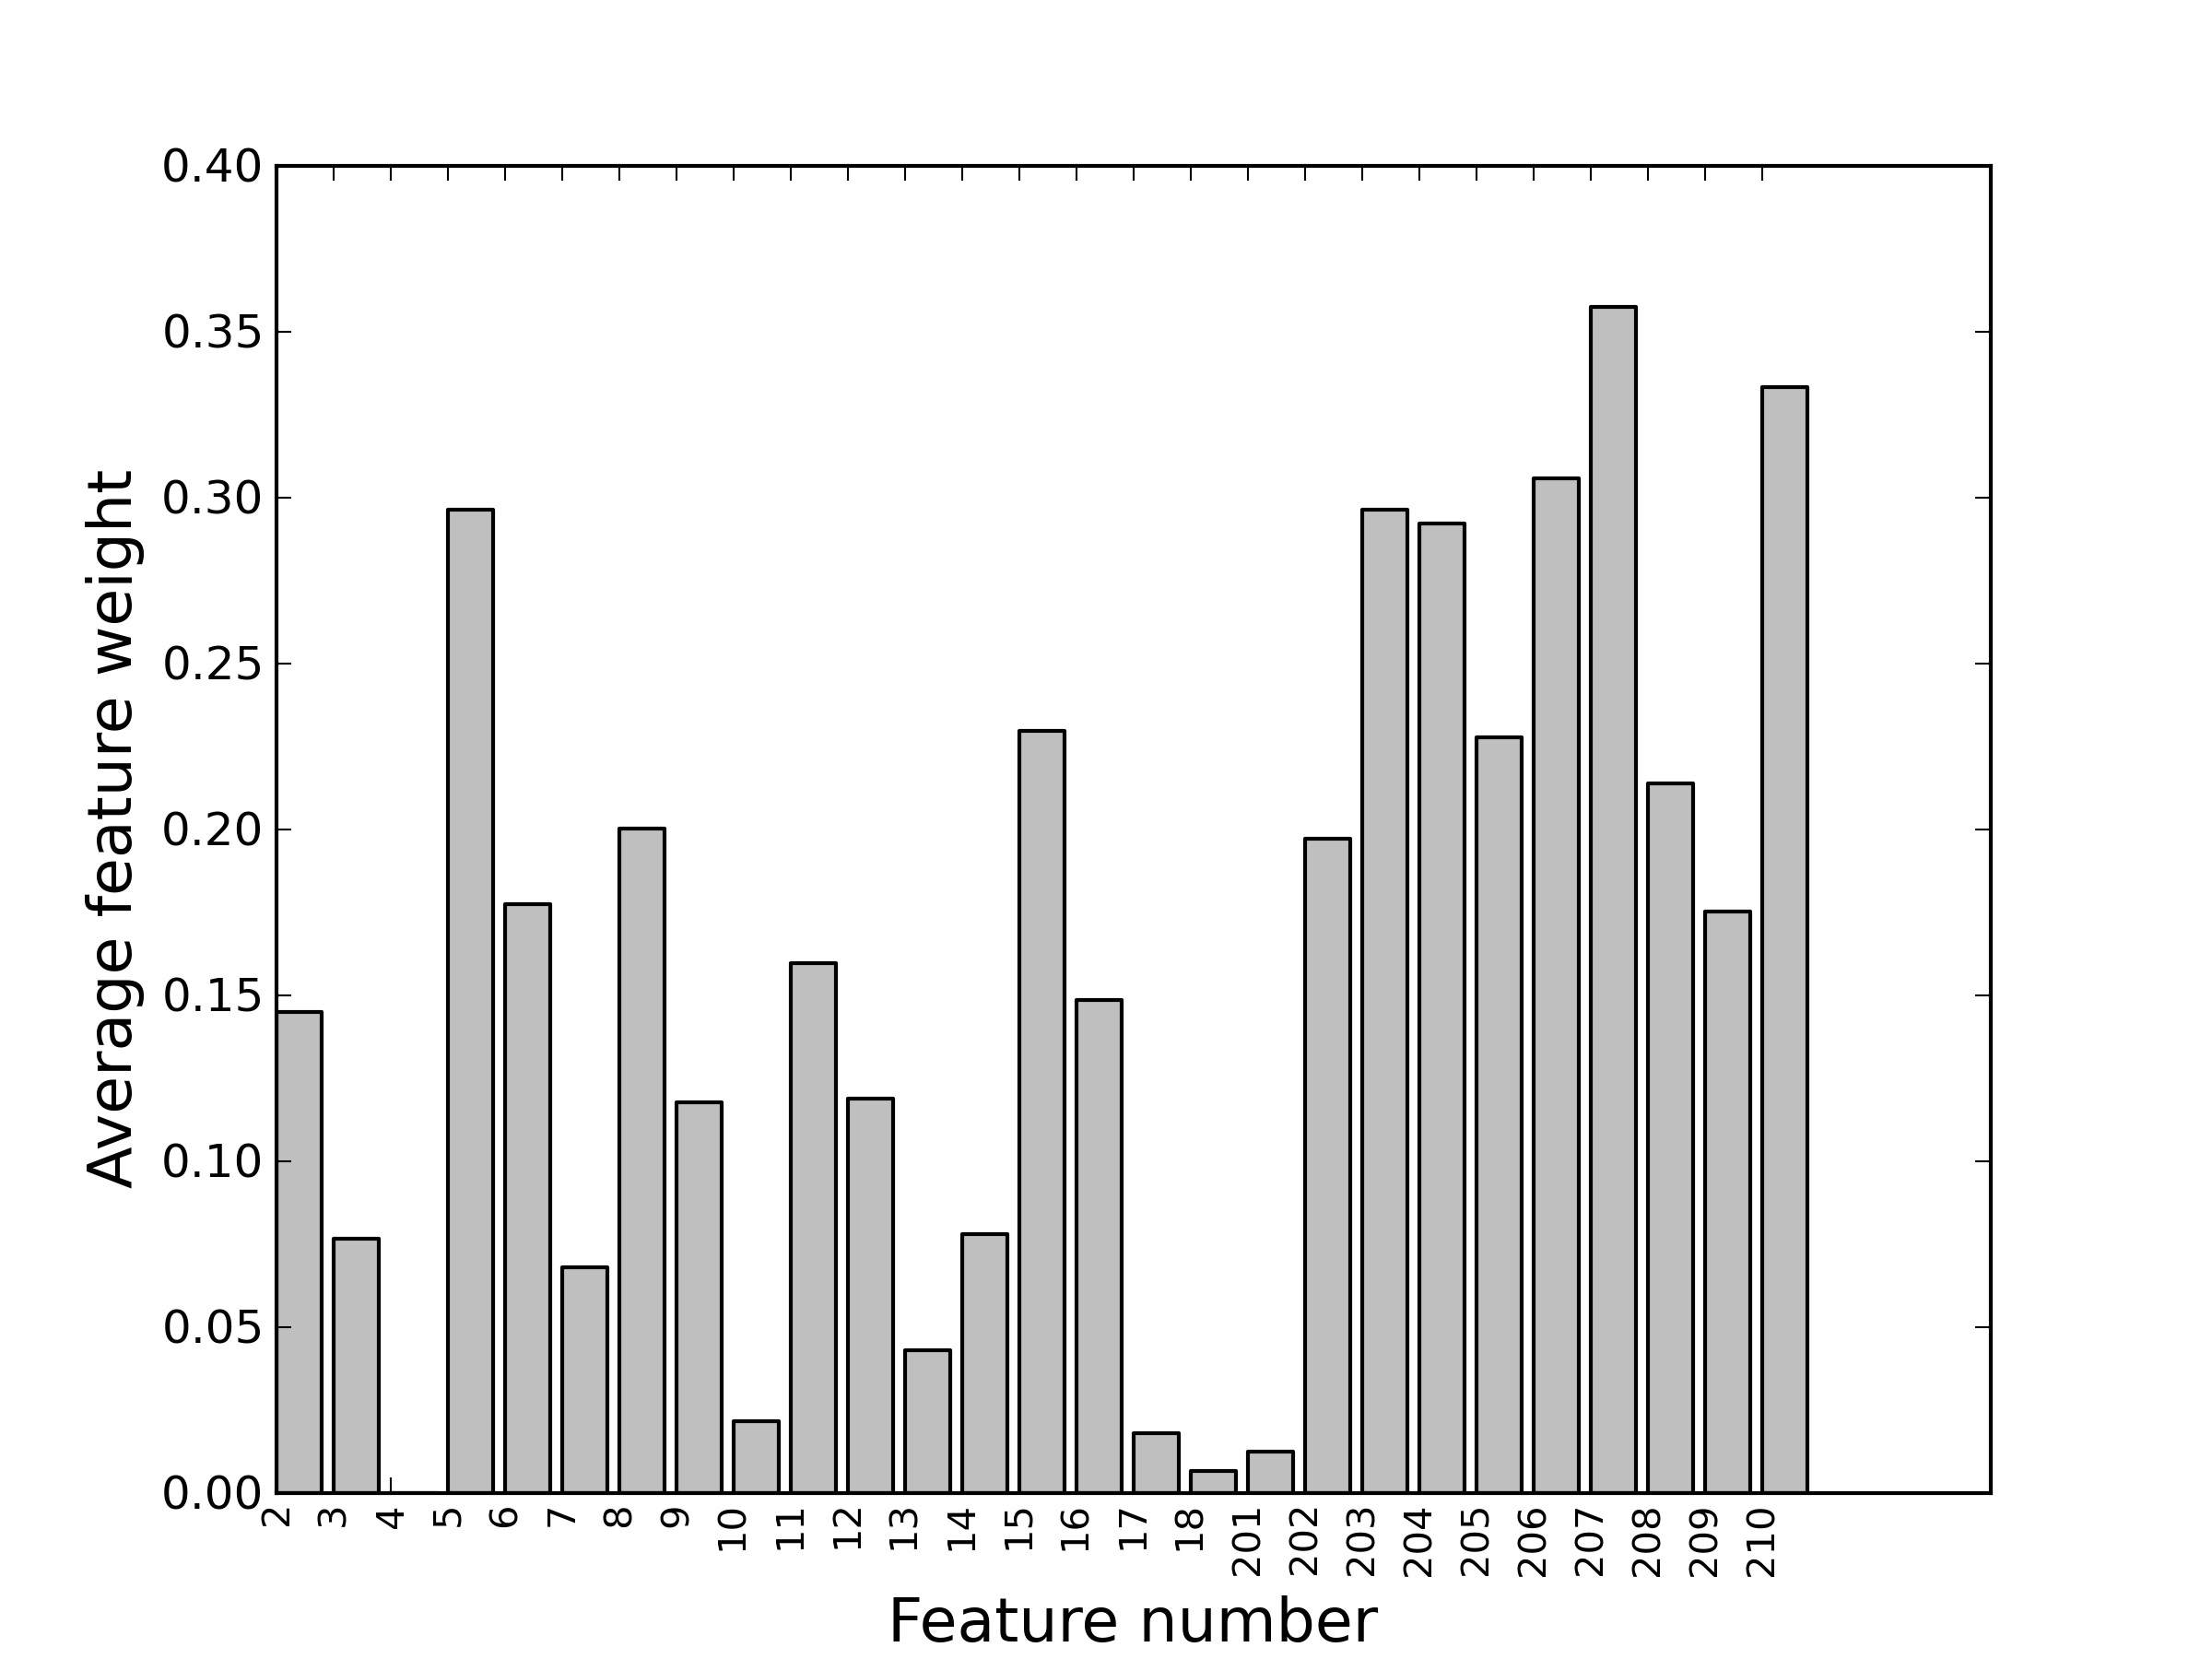
\includegraphics[width=0.7\textwidth]{figures/logreg/randomized_forum_only.png}
\end{figure}

In the both of our smaller cohorts, \both and \wiki, the lab grade (\x{206}) and lab grade over time (\x{207}) are the most predictive features. Although both of these cohorts participated in the Wiki, the number of Wiki edits (\x{4}) actually contains insignificantly small predictive power in both cases. Both cohorts show similar distributions overall. Similar to the larger cohorts, features related to submissions hold the most predictive power.

\begin{figure}[ht!]
  \caption{Feature importances for the \both cohort.}\label{fig:randomized_logistic_regression_forum_and_wiki}
  \centering
    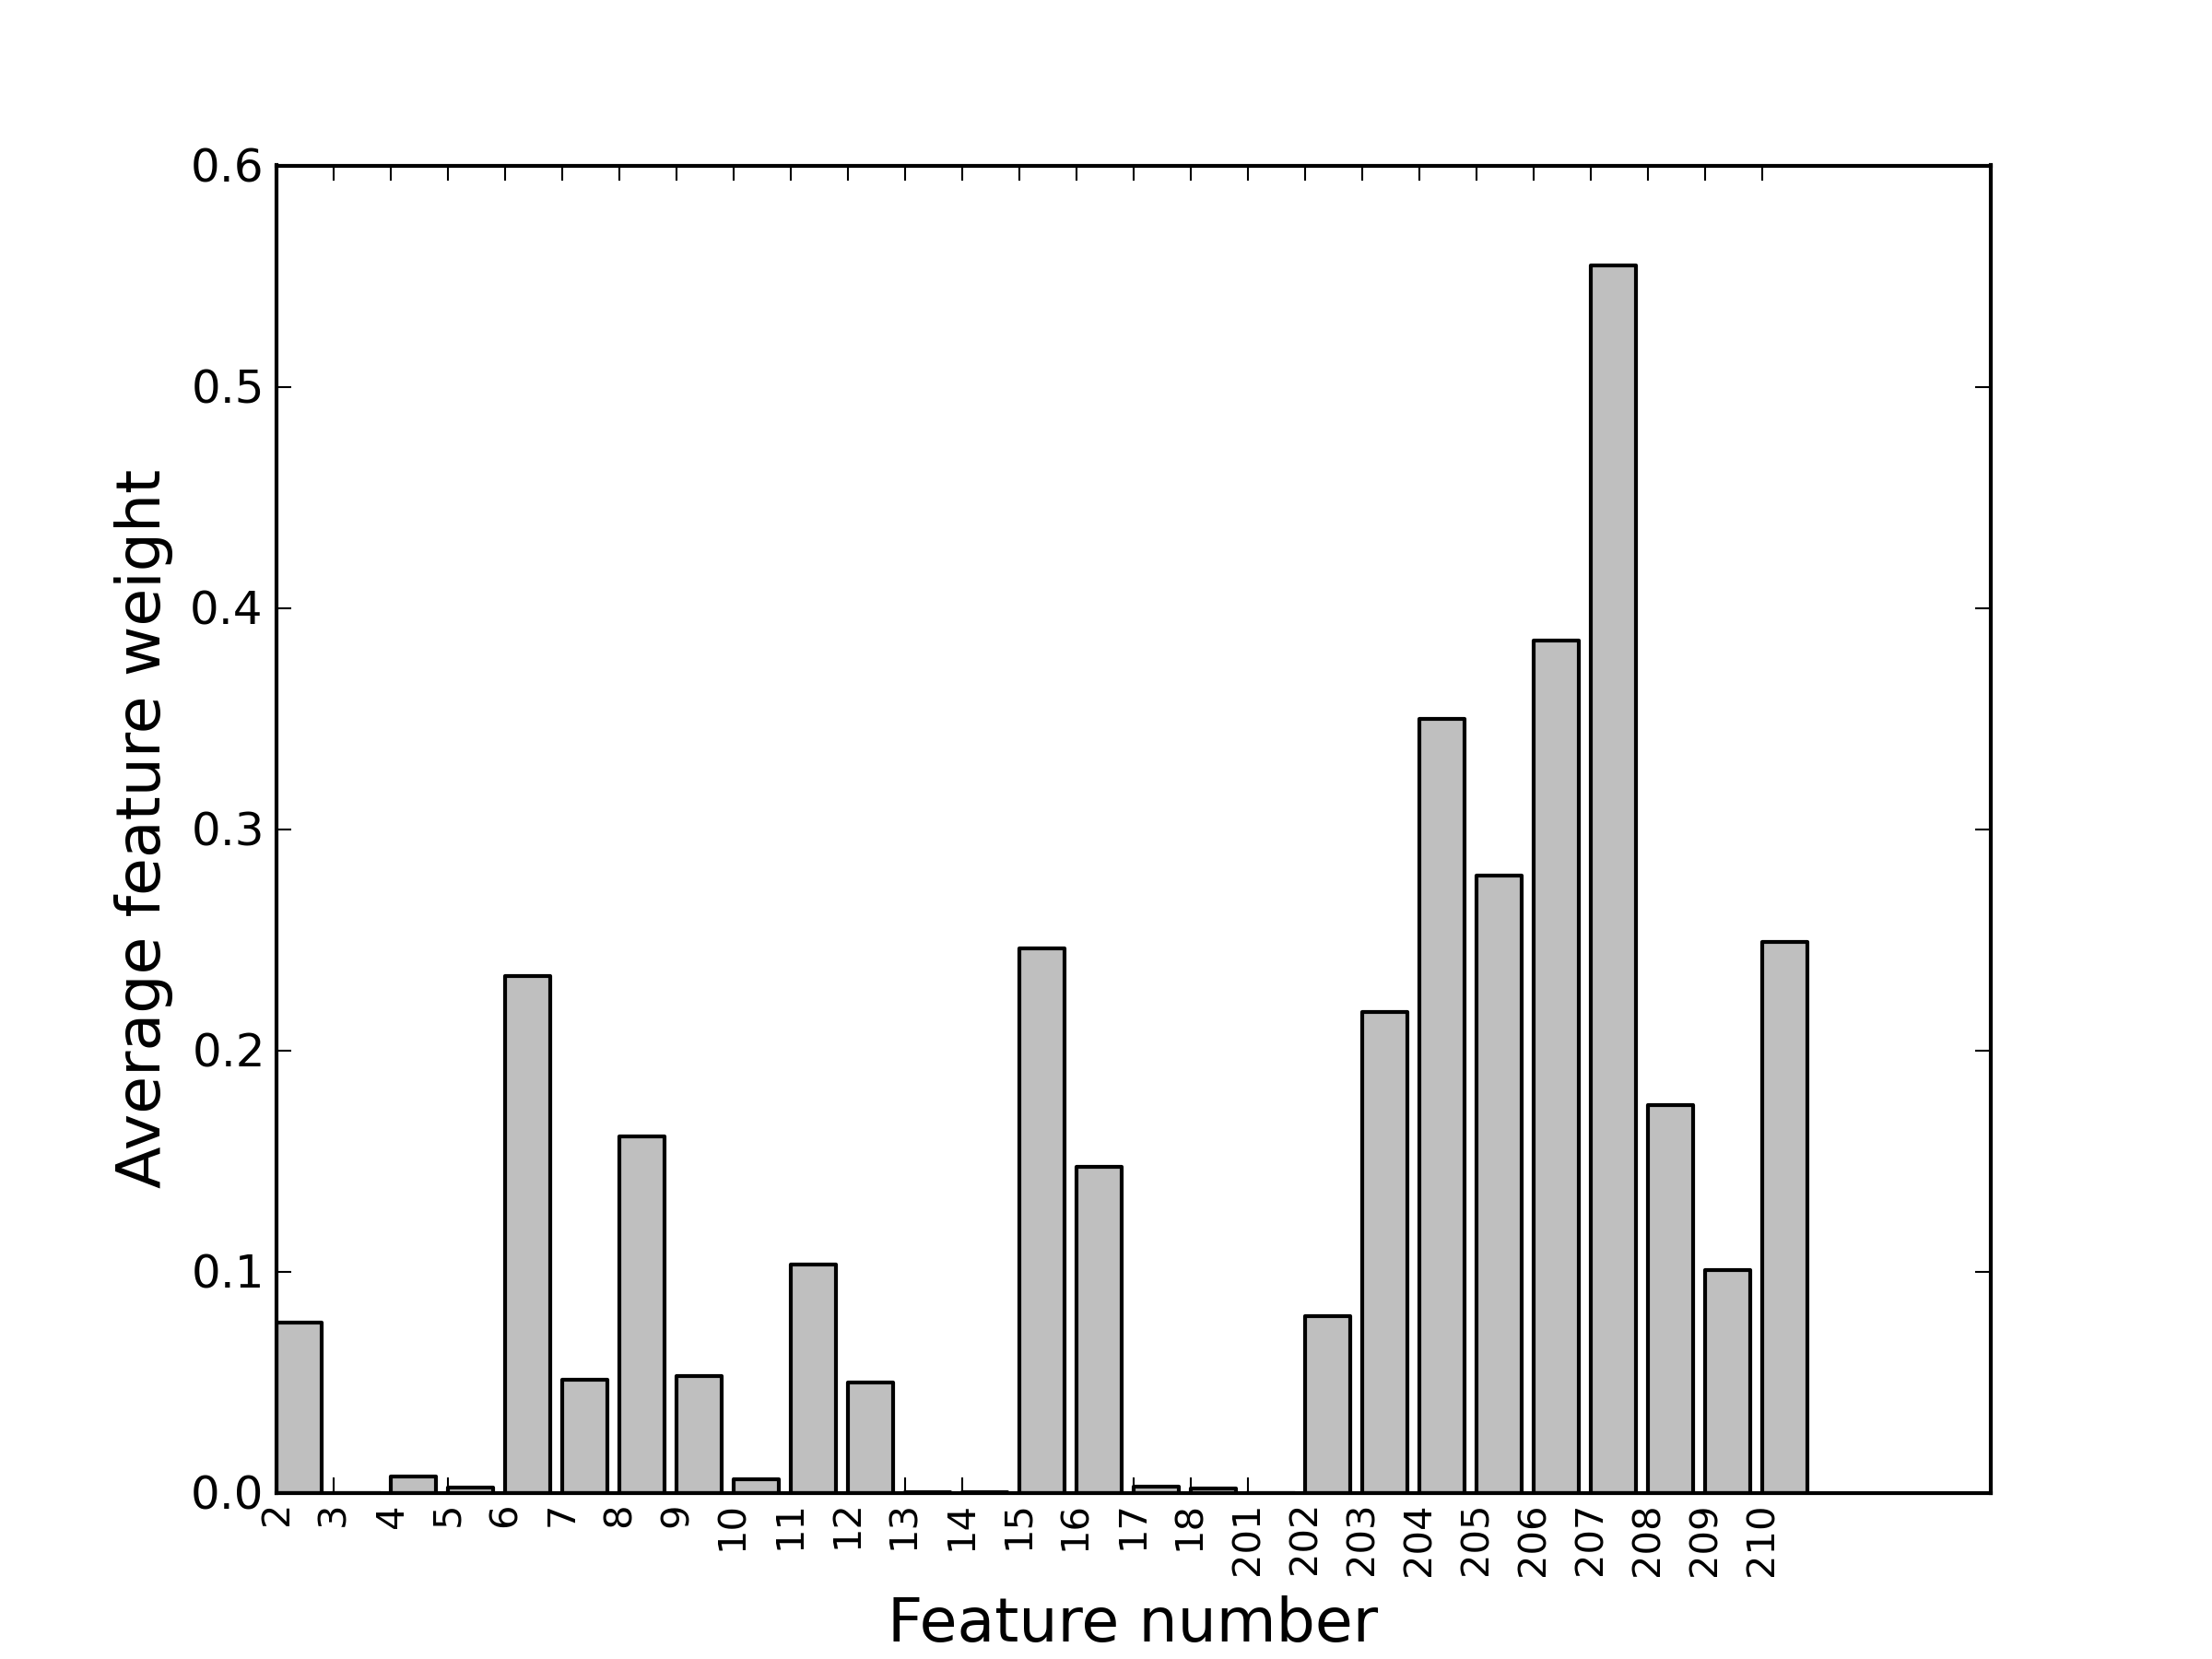
\includegraphics[width=0.7\textwidth]{figures/logreg/randomized_forum_and_wiki.png}
\end{figure}

\begin{figure}[ht!]
  \caption{Feature importances for the \wiki cohort.}\label{fig:randomized_logistic_regression_wiki_only}
  \centering
    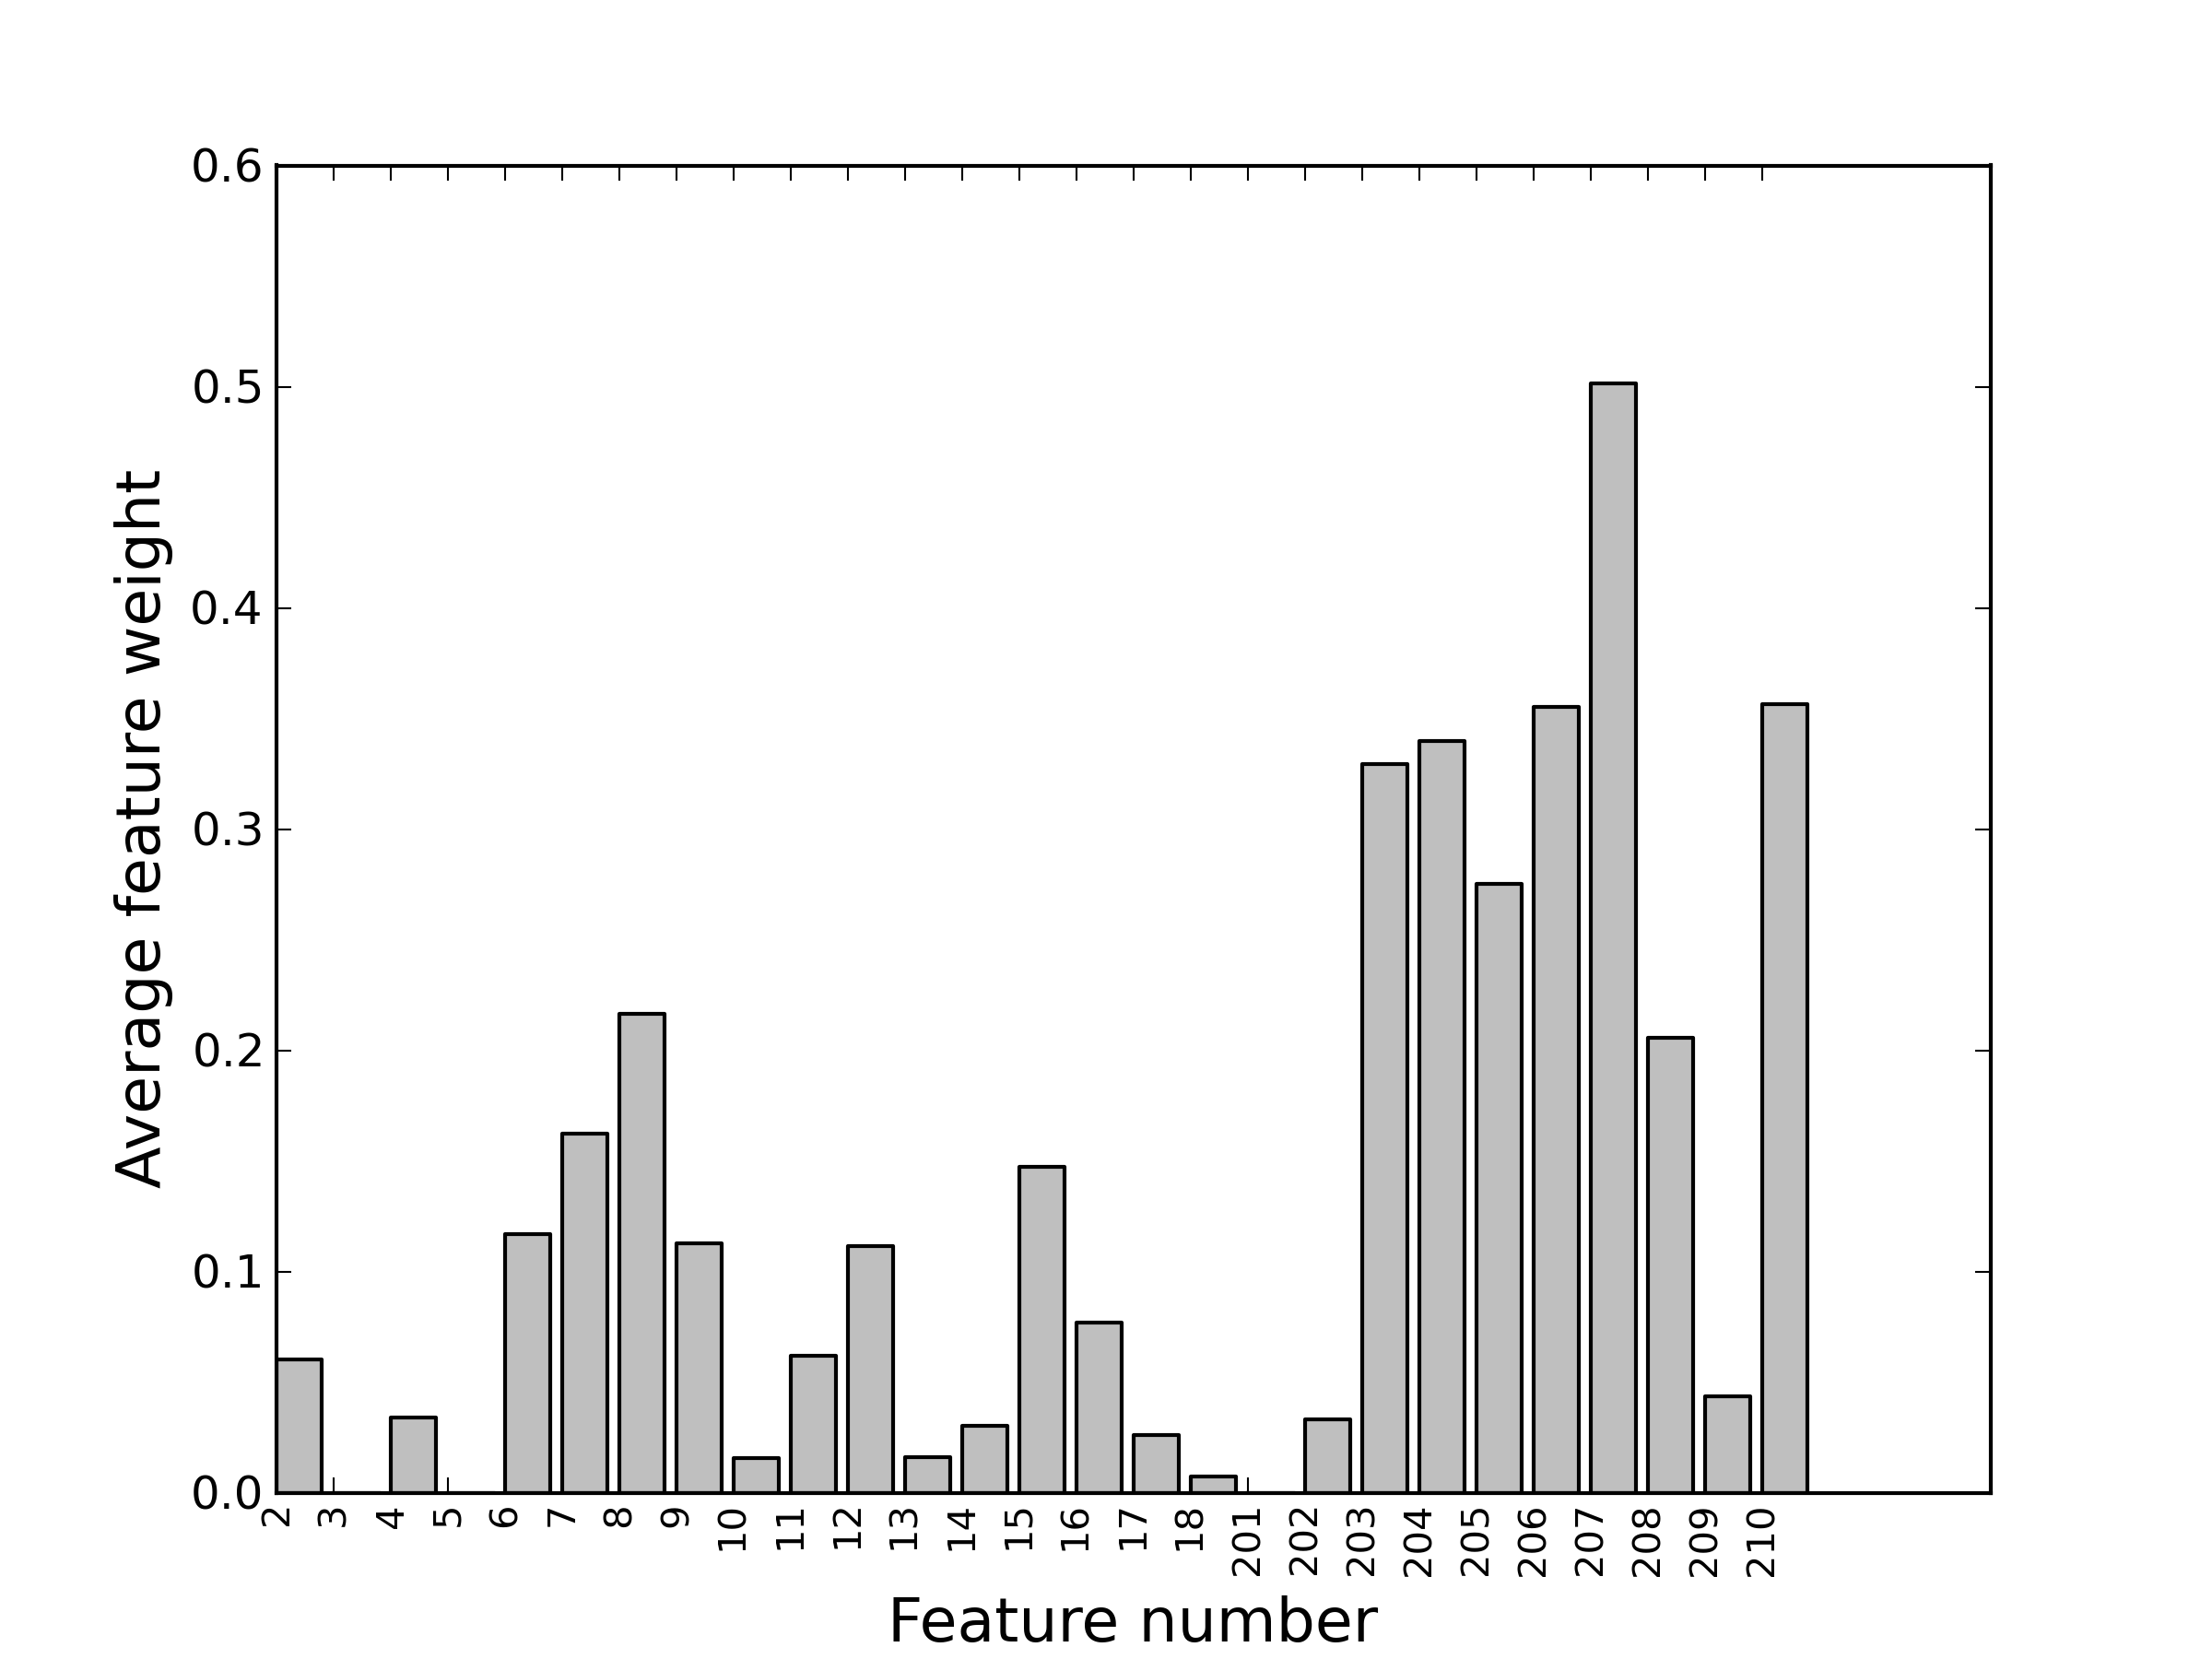
\includegraphics[width=0.7\textwidth]{figures/logreg/randomized_wiki_only.png}
\end{figure}

\end{paragraph}

\begin{paragraph}
{Feature invariant week importance} For any given lag (that is data from weeks 1-to-lag) we wanted to assess which of the week's features (data) are important for a prediction problem. We call this feature-invariant week importance. To evaluate this, we first group the experiments by lag, then for each experiment aggregate the weights for features for each week. We then normalized this value with the total sum of weights. This provided us the relative normalized importance of that week in that experiment. We illustrate this process in Figure~\ref{fig:fiw}. We then repeat this for all the experiments with the same lag and then sum the normalized importances for a week and plot this sum for each lag in the heatmap as shown in the Figure~\ref{fig:randomized_over_time_no_collab}. 

\begin{figure}[ht!]
  \caption{Aggregating different weeks weights to assemble weeks relative importance for a single experiment for a given lag. In this example, the lag is 3. That is,  three weeks data is used to predict a \sti in a future week. The Randomized logistic regression gives the weights for all 27 features for all three weeks (unnormalized). To assemble the feature-invariant relative weight for week 1 we sum the weights for all features in week 1 and divide it with the total weights. We note that this is a heuristic. }\label{fig:fiw}
  \centering
    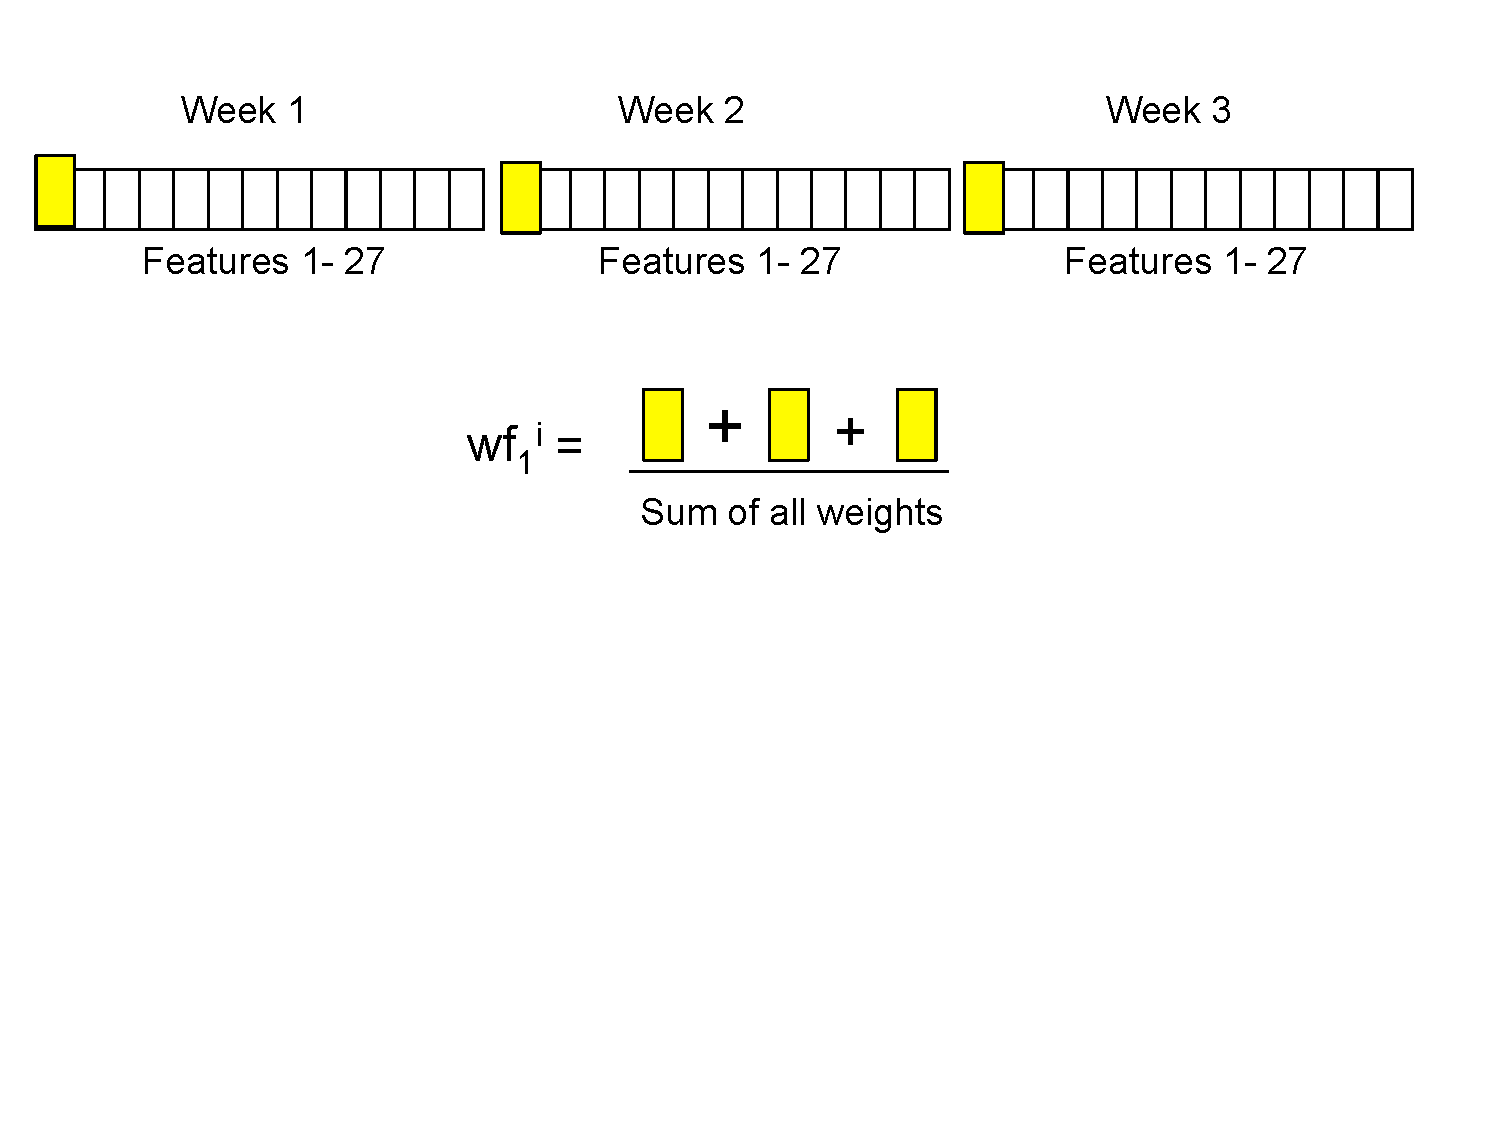
\includegraphics[width=0.6\textwidth]{figures/wif}
\end{figure}


As might be expected, most feature vectors used only more recent weeks of data in order to predict. For example, for the \neither cohort, for a \lag of 8, predicted week of 11, the majority of the first 6 weeks of data have no feature weight, and the nonzero weights are all below 0.15, whereas features of week 10 include weights as large as 0.965 (for \x{11}). Figures \ref{fig:randomized_over_time_no_collab} through \ref{fig:randomized_over_time_wiki_only} show a heatmap of these results.

\begin{figure}[ht!]
  \caption{Feature week's importance as \lag varies for the \neither cohort.}\label{fig:randomized_over_time_no_collab}
  \centering
    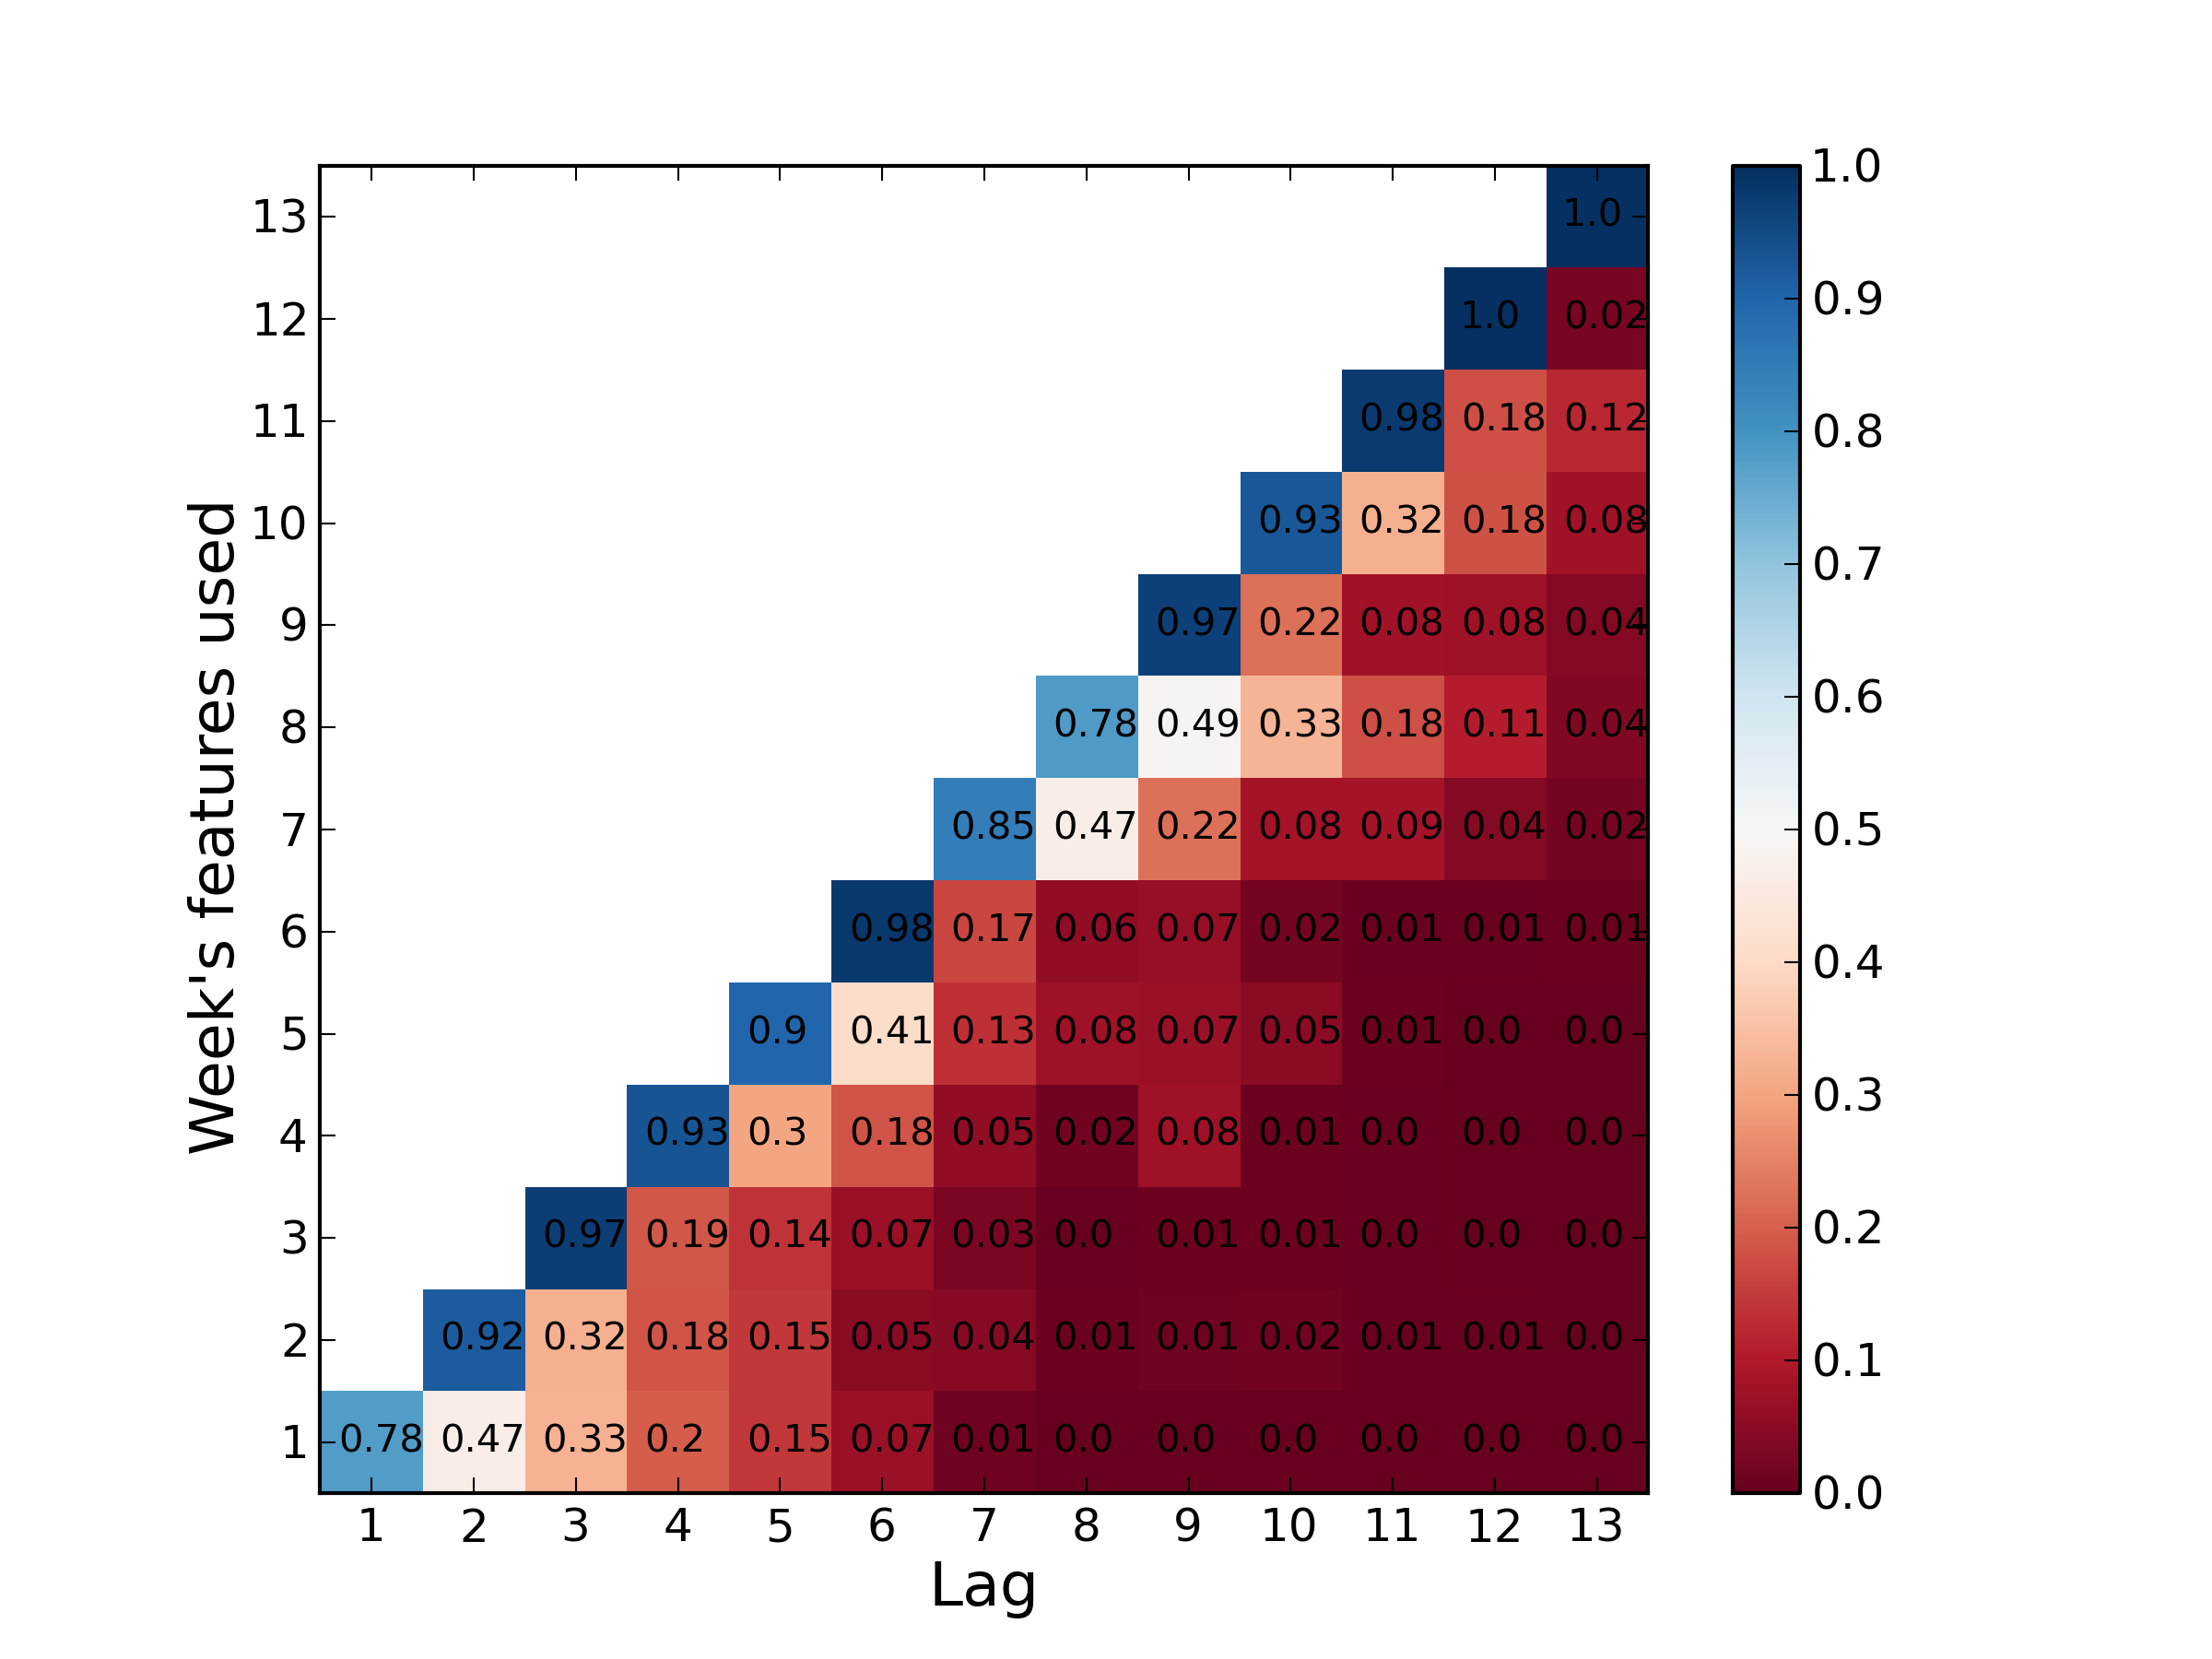
\includegraphics[width=0.9\textwidth]{figures/logreg/randomized_no_collab_over_time.png}
\end{figure}

\begin{figure}[ht!]
  \caption{Feature week's importance as \lag varies for the \forum cohort.}\label{fig:randomized_over_time_forum_only}
  \centering
    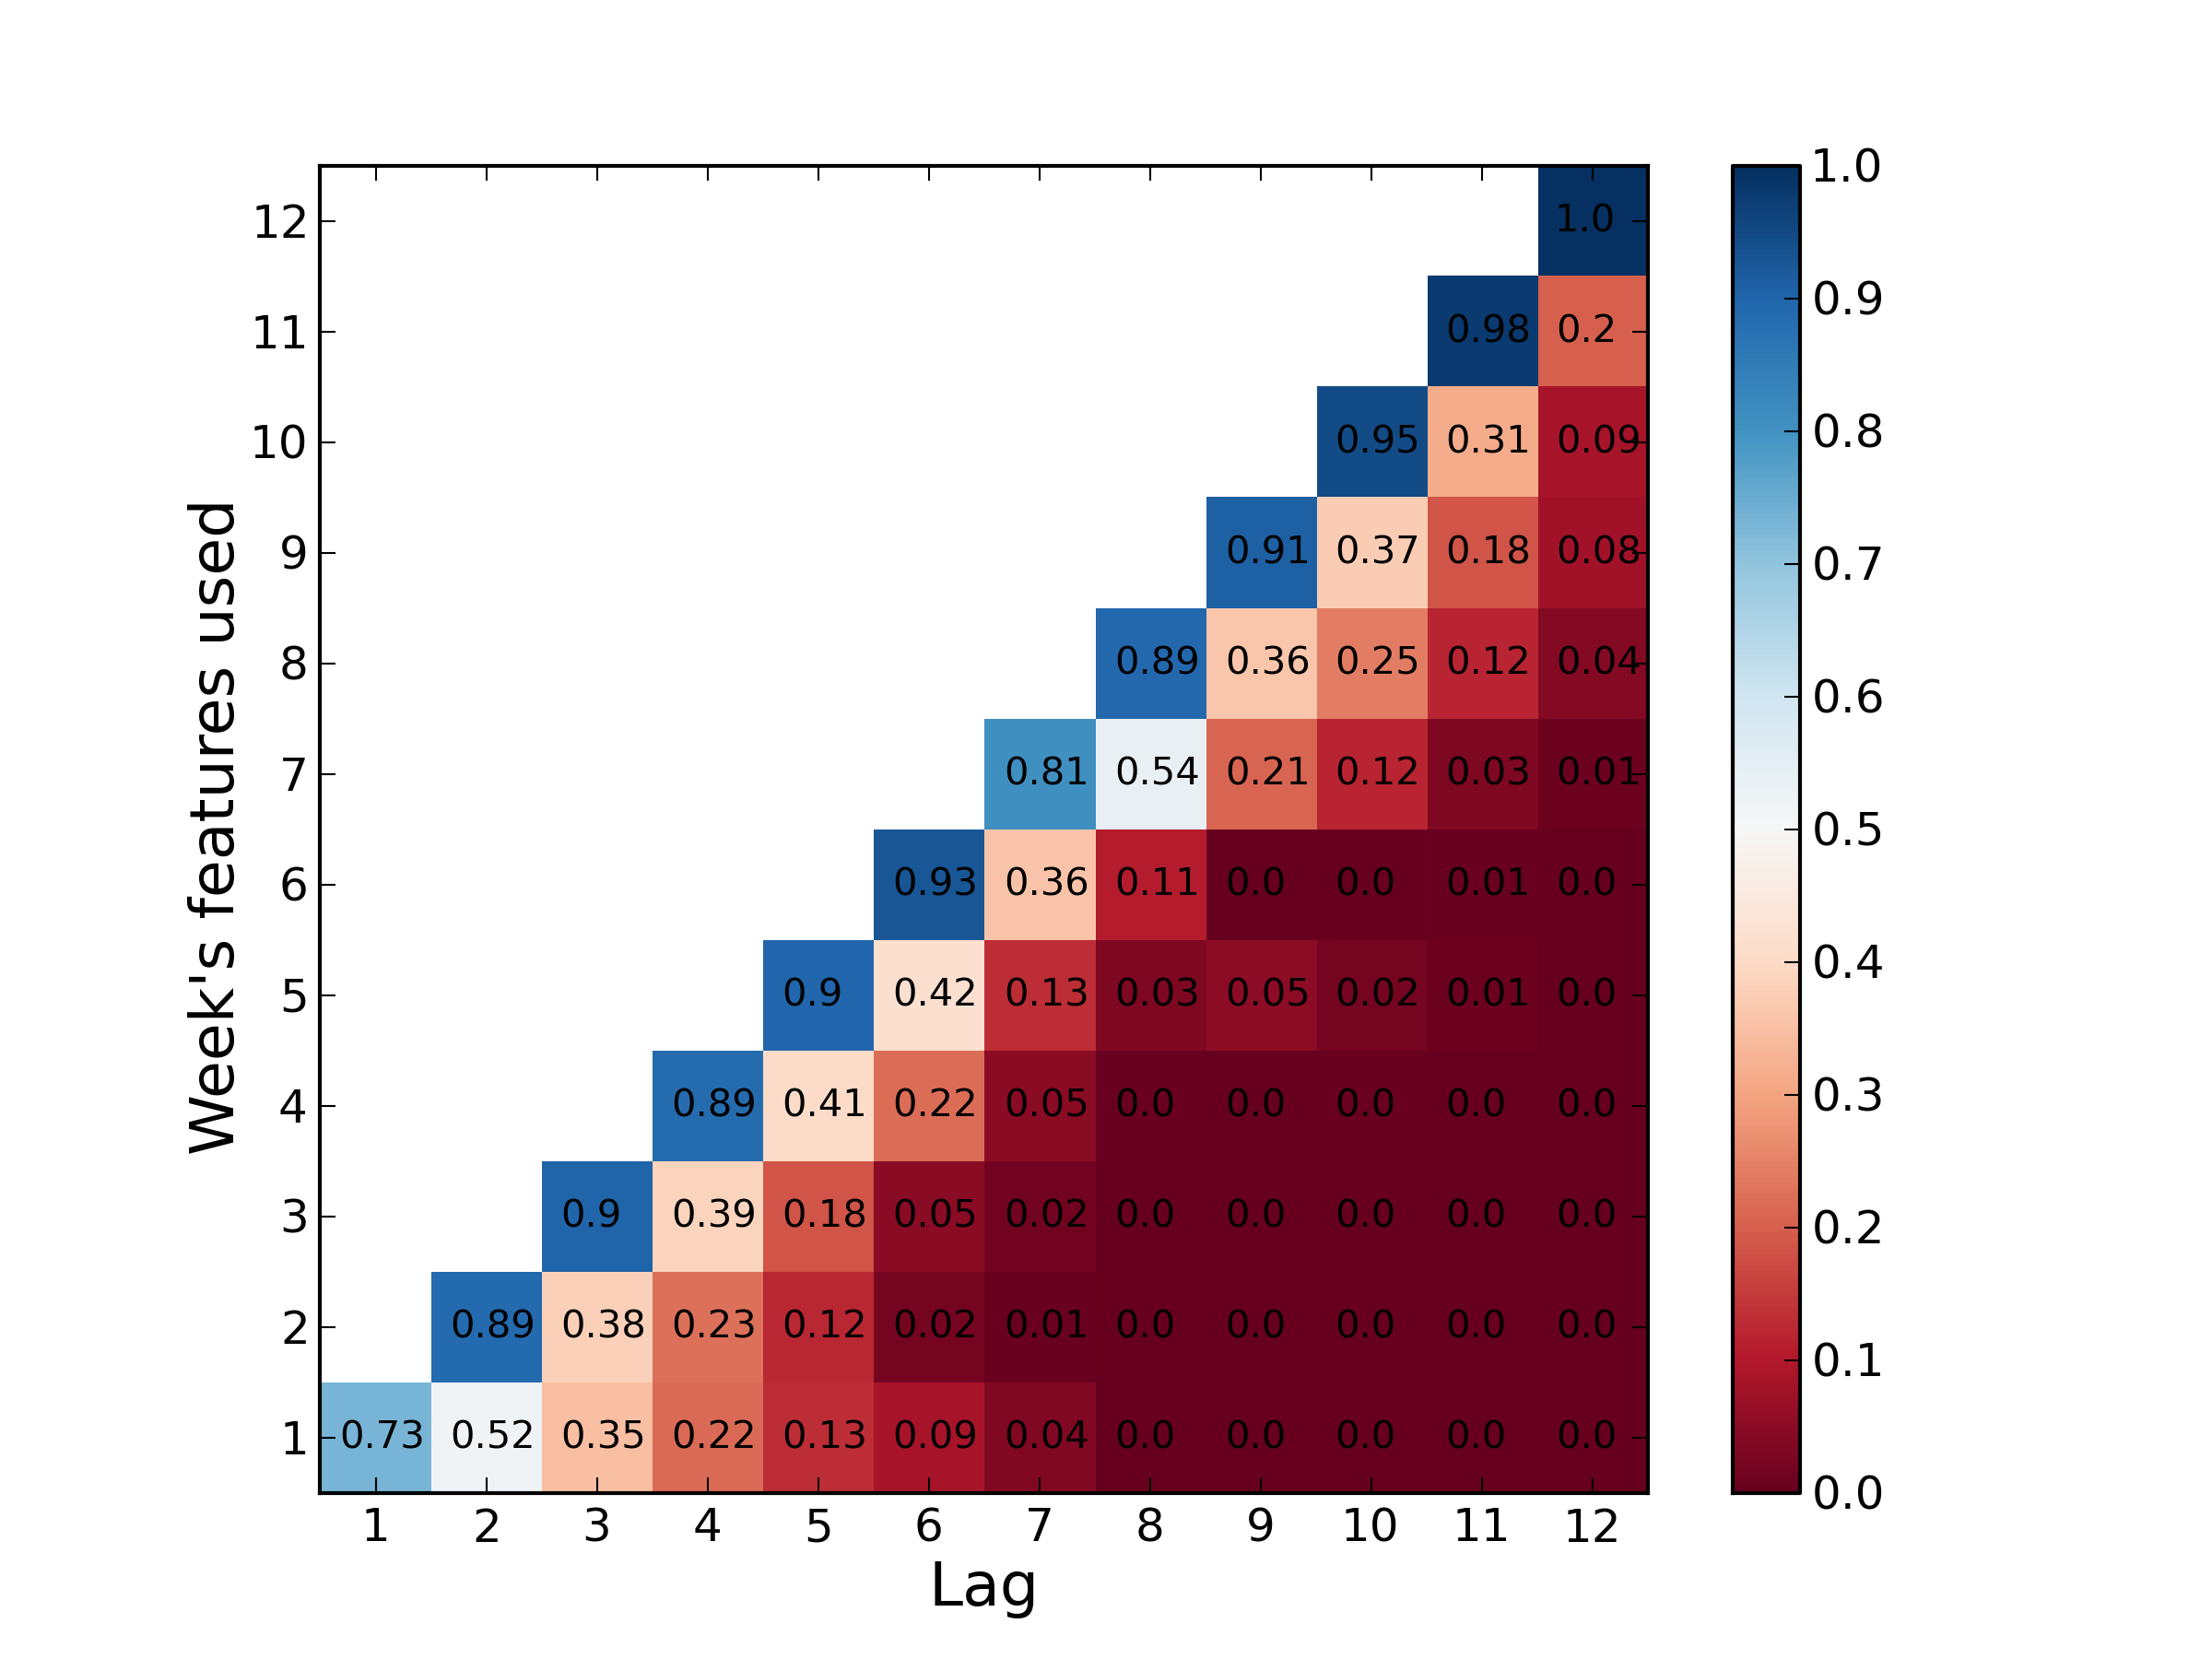
\includegraphics[width=0.9\textwidth]{figures/logreg/randomized_forum_only_over_time.png}
\end{figure}

\begin{figure}[ht!]
  \caption{Feature week's importance as \lag varies for the \both cohort.}\label{fig:randomized_over_time_forum_and_wiki}
  \centering
    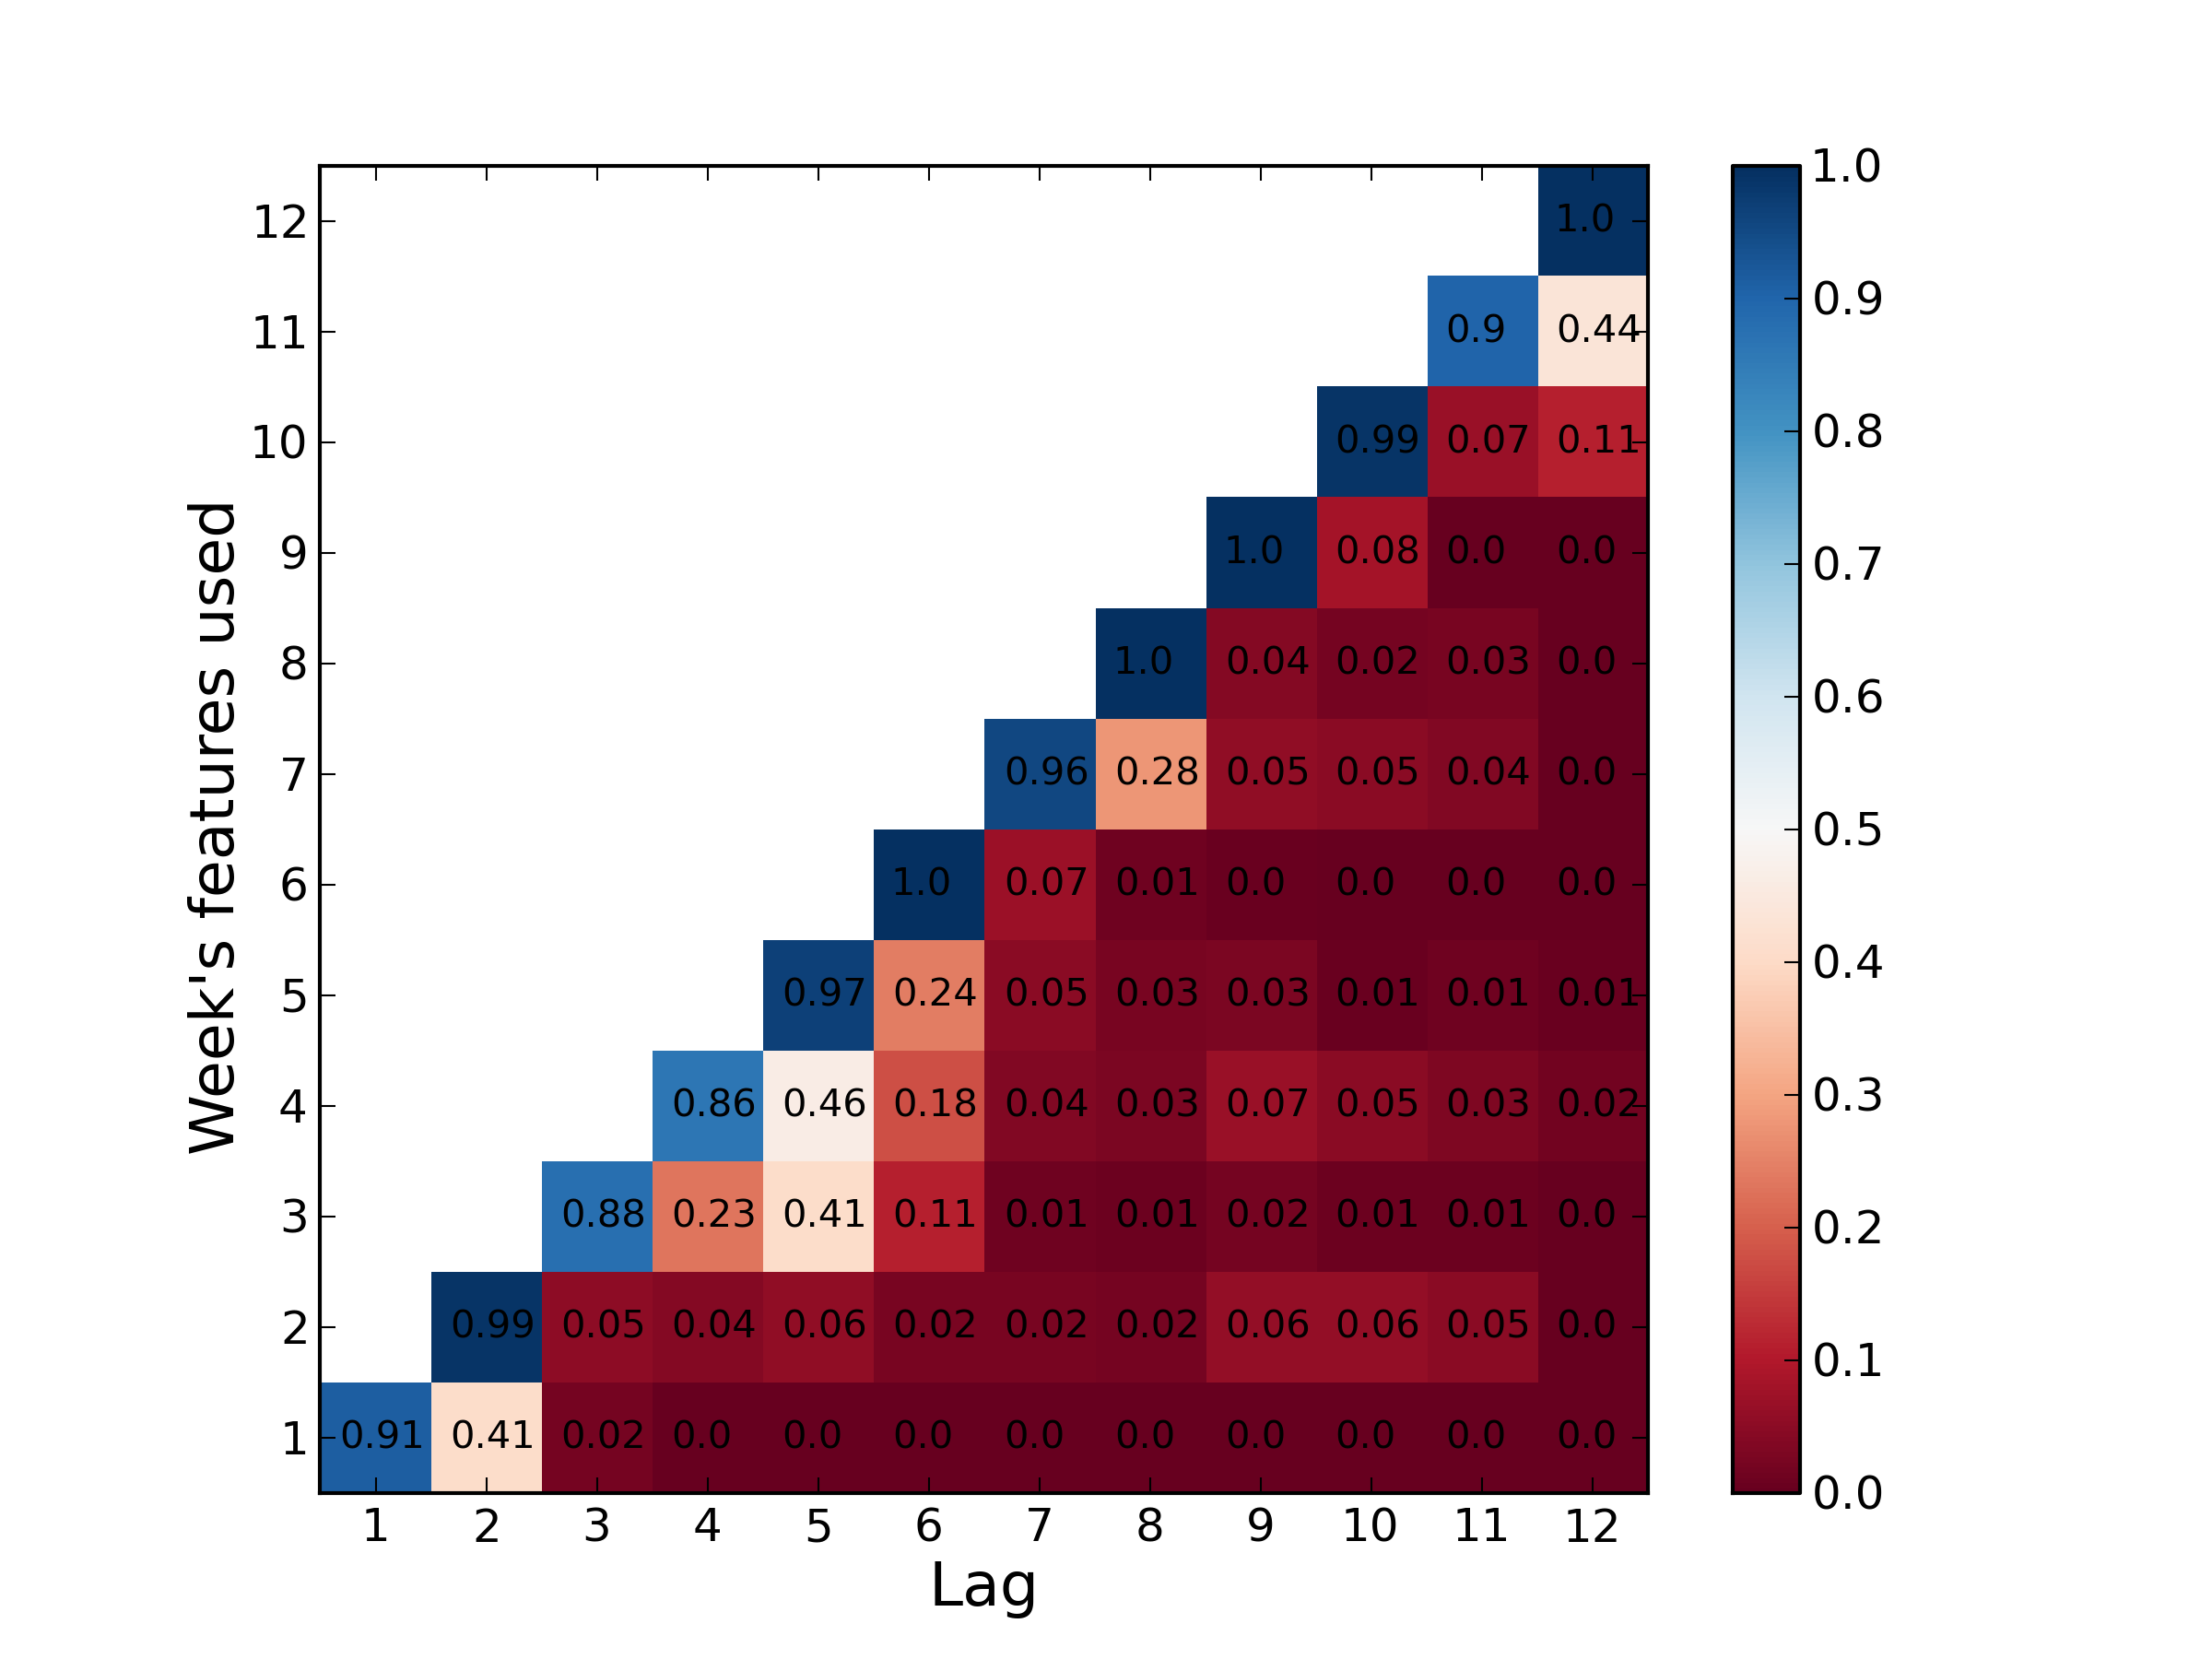
\includegraphics[width=0.9\textwidth]{figures/logreg/randomized_forum_and_wiki_over_time.png}
\end{figure}

\begin{figure}[ht!]
  \caption{Feature week's importance as \lag varies for the \wiki cohort.}\label{fig:randomized_over_time_wiki_only}
  \centering
    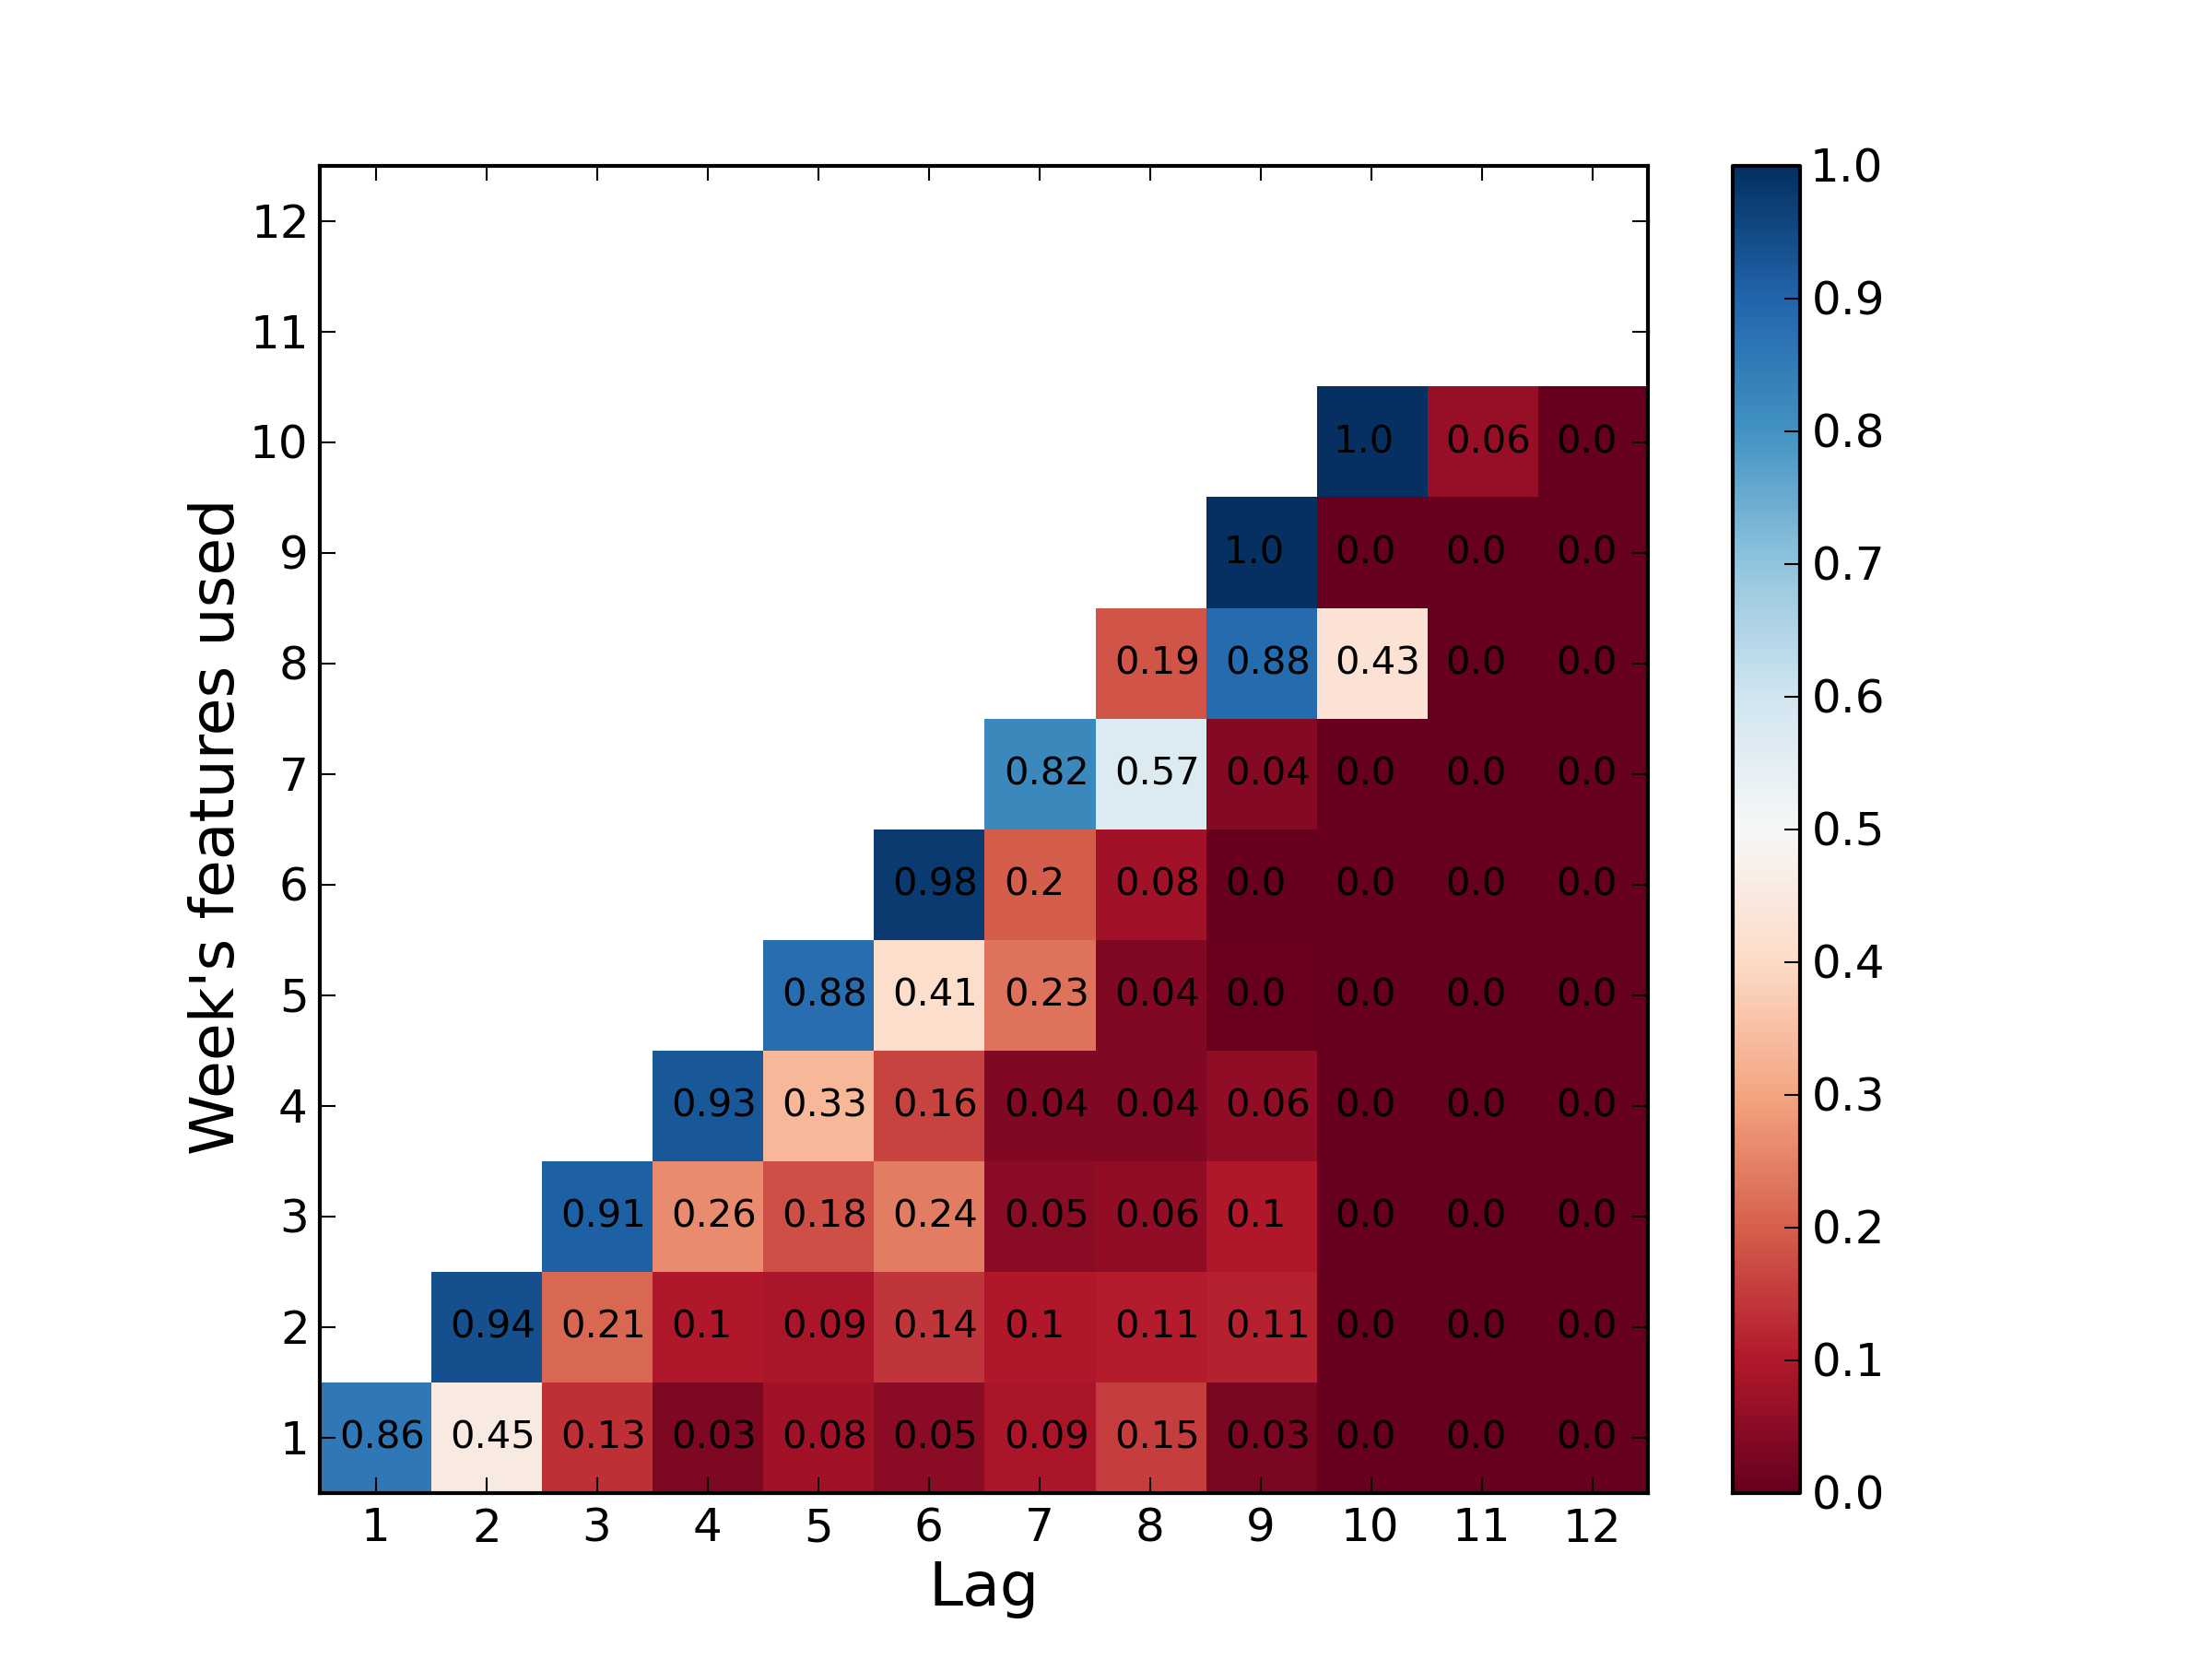
\includegraphics[width=0.9\textwidth]{figures/logreg/randomized_wiki_only_over_time.png}
\end{figure}

As expected, for each \lag, the week's features that mattered the most are the final weeks. This quickly drops off. For each cohort, the logistic regression models use approximately the last four weeks of data, regardless of the \lag. This indicates that there is not much added value in using more than four weeks of data as the \lag increases. This information would be useful when prediction must be done quickly, such as in real-time analytics.

\end{paragraph}




